\documentclass[a4paper,14pt,oneside,openany]{memoir}

\tolerance10000
\hbadness10000

%%% Задаем поля, отступы и межстрочный интервал %%%

\usepackage[left=30mm, right=10mm, top=20mm, bottom=20mm]{geometry} % Пакет geometry с аргументами для определения полей
\pagestyle{plain} % Убираем стандарные для данного класса верхние колонтитулы с заголовком текущей главы, оставляем только номер страницы снизу по центру
\parindent=1cm % Абзацный отступ 1.25 см, приблизительно равно пяти знакам, как по ГОСТ
\usepackage{indentfirst} % Добавляем отступ к первому абзацу
%\linespread{1.3} % Межстрочный интервал (наиболее близко к вордовскому полуторному) - тут вместо этого используется команда OnehalfSpacing*

%%% Задаем языковые параметры и шрифт %%%

\usepackage[english, russian]{babel}                % Настройки для русского языка как основного в тексте
\babelfont{rm}{Times New Roman}                     % TMR в качестве базового roman-щрифта

%%% Задаем стиль заголовков и подзаголовков в тексте %%%

\setsecnumdepth{subsection} % Номера разделов считать до третьего уровня включительно, т.е. нумеруются только главы, секции, подсекции
\renewcommand*{\chapterheadstart}{} % Переопределяем команду, задающую отступ над заголовком, чтобы отступа не было
% \newcommand{\chapterfont}{\fontsize{14pt}{16pt}\selectfont}
% \renewcommand*{\printchaptername}{} % Переопределяем команду, печатающую слово "Глава", чтобы оно не печалось
%\renewcommand*{\printchapternum}{} % То же самое для номера главы - тут не надо, номер главы оставляем
\renewcommand*{\chapnumfont}{\large\bfseries} % Меняем стиль шрифта для номера главы: нормальный размер, полужирный
\renewcommand*{\chapnamefont}{\large\bfseries} % Меняем стиль шрифта для номера главы: нормальный размер, полужирный
\renewcommand*{\afterchapternum}{\hspace{1em}} % Меняем разделитель между номером главы и названием
\renewcommand*{\printchaptertitle}{\large\bfseries\centering} % Меняем стиль написания для заголовка главы: нормальный размер, полужирный, центрированный
\setbeforesecskip{20pt} % Задаем отступ перед заголовком секции
\setaftersecskip{20pt} % Ставим такой же отступ после заголовка секции
\setsecheadstyle{\raggedright\normalfont\bfseries} % Меняем стиль написания для заголовка секции: выравнивание по правому краю без переносов, нормальный размер, полужирный
\setbeforesubsecskip{20pt} % Задаем отступ перед заголовком подсекции
\setaftersubsecskip{20pt} % Ставим такой же отступ после заголовка подсекции
\setsubsecheadstyle{\raggedright\normalfont\bfseries}  % Меняем стиль написания для заголовка подсекции: выравнивание по правому краю без переносов, нормальный размер, полужирный

%%% Задаем параметры оглавления %%%

\setrmarg{2.55em plus1fil} % Запрещаем переносы слов в оглавлении
%\setlength{\cftbeforechapterskip}{0pt} % Эта команда убирает интервал между заголовками глав - тут не надо, так красивее смотрится
\renewcommand{\aftertoctitle}{\afterchaptertitle \vspace{-\cftbeforechapterskip}} % Делаем отступ между словом "Содержание" и первой строкой таким же, как у заголовков глав
\renewcommand*{\chapternumberline}[1]{} % Делаем так, чтобы номер главы не печатался - тут не надо
\renewcommand*{\cftchapternumwidth}{1.5em} % Ставим подходящий по размеру разделитель между номером главы и самим заголовком
\renewcommand*{\cftchapterfont}{\normalfont} % Названия глав обычным шрифтом заглавными буквами
\renewcommand*{\cftchapterpagefont}{\normalfont} % Номера страниц обычным шрифтом
\renewcommand*{\cftchapterdotsep}{\cftdotsep} % Делаем точки до номера страницы после названий глав
\renewcommand*{\cftdotsep}{1} % Задаем расстояние между точками
\renewcommand*{\cftchapterleader}{\cftdotfill{\cftchapterdotsep}} % Делаем точки стандартной формы (по умолчанию они "жирные")
\renewcommand*{\baselinestretch}{1.3} % Межстрочный интервал 
\maxtocdepth{subsection} % В оглавление попадают только разделы первых трех уровней: главы, секции и подсекции

%%% Выравнивание и переносы %%%

%% http://tex.stackexchange.com/questions/241343/what-is-the-meaning-of-fussy-sloppy-emergencystretch-tolerance-hbadness
%% http://www.latex-community.org/forum/viewtopic.php?p=70342#p70342
\tolerance 1414
\hbadness 1414
\emergencystretch 1.5em                             % В случае проблем регулировать в первую очередь
\hfuzz 0.3pt
\vfuzz \hfuzz
%\dbottom
%\sloppy                                            % Избавляемся от переполнений
\clubpenalty=10000                                  % Запрещаем разрыв страницы после первой строки абзаца
\widowpenalty=10000                                 % Запрещаем разрыв страницы после последней строки абзаца
\brokenpenalty=4991                                 % Ограничение на разрыв страницы, если строка заканчивается переносом

%%% Объясняем компилятору, какие буквы русского алфавита можно использовать в перечислениях (подрисунках и нумерованных списках) %%%
%%% По ГОСТ нельзя использовать буквы ё, з, й, о, ч, ь, ы, ъ %%%
%%% Здесь также переопределены заглавные буквы, хотя в принципе они в документе не используются %%%

\makeatletter
    \def\russian@Alph#1{\ifcase#1\or
       А\or Б\or В\or Г\or Д\or Е\or Ж\or
       И\or К\or Л\or М\or Н\or
       П\or Р\or С\or Т\or У\or Ф\or Х\or
       Ц\or Ш\or Щ\or Э\or Ю\or Я\else\xpg@ill@value{#1}{russian@Alph}\fi}
    \def\russian@alph#1{\ifcase#1\or
       а\or б\or в\or г\or д\or е\or ж\or
       и\or к\or л\or м\or н\or
       п\or р\or с\or т\or у\or ф\or х\or
       ц\or ш\or щ\or э\or ю\or я\else\xpg@ill@value{#1}{russian@alph}\fi}
\makeatother

%%% Задаем параметры оформления рисунков и таблиц %%%

\usepackage{graphicx, caption, subcaption} % Подгружаем пакеты для работы с графикой и настройки подписей
\graphicspath{{src/}} % Определяем папку с рисунками
\captionsetup[figure]{font=small, width=\textwidth, name=Рисунок, justification=centering} % Задаем параметры подписей к рисункам: маленький шрифт (в данном случае 12pt), ширина равна ширине текста, полнотекстовая надпись "Рисунок", выравнивание по центру
% \captionsetup[subfigure]{font=small} % Индексы подрисунков а), б) и так далее тоже шрифтом 12pt (по умолчанию делает еще меньше)
% \captionsetup[table]{singlelinecheck=false,font=small,width=\textwidth,justification=justified} % Задаем параметры подписей к таблицам: запрещаем переносы, маленький шрифт (в данном случае 12pt), ширина равна ширине текста, выравнивание по ширине
\captiondelim{ --- } % Разделителем между номером рисунка/таблицы и текстом в подписи является длинное тире
\setkeys{Gin}{width=\textwidth} % По умолчанию размер всех добавляемых рисунков будет подгоняться под ширину текста
\renewcommand{\thesubfigure}{\asbuk{subfigure}} % Нумерация подрисунков строчными буквами кириллицы
%\setlength{\abovecaptionskip}{0pt} % Отбивка над подписью - тут не меняем
%\setlength{\belowcaptionskip}{0pt} % Отбивка под подписью - тут не меняем
\usepackage[section]{placeins} % Объекты типа float (рисунки/таблицы) не вылезают за границы секциии, в которой они объявлены

%%% Задаем параметры ссылок и гиперссылок %%% 

\usepackage{hyperref}                               % Подгружаем нужный пакет
\hypersetup{
    colorlinks=true,                                % Все ссылки и гиперссылки цветные
    linktoc=all,                                    % В оглавлении ссылки подключатся для всех отображаемых уровней
    linktocpage=true,                               % Ссылка - только номер страницы, а не весь заголовок (так выглядит аккуратнее)
    linkcolor=black,                                  % Цвет ссылок и гиперссылок - красный
    citecolor=black                                   % Цвет цитировний - красный
}

%%% Настраиваем отображение списков %%%

\usepackage{enumitem}                               % Подгружаем пакет для гибкой настройки списков
\renewcommand*{\labelitemi}{\normalfont{--}}        % В ненумерованных списках для пунктов используем короткое тире
\makeatletter
    \AddEnumerateCounter{\asbuk}{\russian@alph}     % Объясняем пакету enumitem, как использовать asbuk
\makeatother
\renewcommand{\labelenumii}{\asbuk{enumii})}        % Кириллица для второго уровня нумерации
\renewcommand{\labelenumiii}{\arabic{enumiii})}     % Арабские цифры для третьего уровня нумерации
\setlist{noitemsep, leftmargin=*}                   % Убираем интервалы между пунками одного уровня в списке
\setlist[1]{labelindent=\parindent}                 % Отступ у пунктов списка равен абзацному отступу
\setlist[2]{leftmargin=\parindent}                  % Плюс еще один такой же отступ для следующего уровня
\setlist[3]{leftmargin=\parindent}                  % И еще один для третьего уровня

%%% Счетчики для нумерации объектов %%%

\counterwithout{figure}{chapter}                    % Сквозная нумерация рисунков по документу
\counterwithout{equation}{chapter}                  % Сквозная нумерация математических выражений по документу
\counterwithout{table}{chapter}                     % Сквозная нумерация таблиц по документу

%%% Реализация библиографии пакетами biblatex и biblatex-gost с использованием движка biber %%%

\usepackage{csquotes} % Пакет для оформления сложных блоков цитирования (biblatex рекомендует его подключать)
\usepackage[%
backend=biber,                                      % Движок
bibencoding=utf8,                                   % Кодировка bib-файла
sorting=none,                                       % Настройка сортировки списка литературы
style=gost-numeric,                                 % Стиль цитирования и библиографии по ГОСТ
language=auto,                                      % Язык для каждой библиографической записи задается отдельно
autolang=other,                                     % Поддержка многоязычной библиографии
sortcites=true,                                     % Если в квадратных скобках несколько ссылок, то отображаться будут отсортированно
movenames=false,                                    % Не перемещать имена, они всегда в начале библиографической записи
maxnames=5,                                         % Максимальное отображаемое число авторов
minnames=3,                                         % До скольки сокращать число авторов, если их больше максимума
doi=false,                                          % Не отображать ссылки на DOI
isbn=false,                                         % Не показывать ISBN, ISSN, ISRN
]{biblatex}[2016/09/17]
\DeclareDelimFormat{bibinitdelim}{}                 % Убираем пробел между инициалами (Иванов И.И. вместо Иванов И. И.)
\addbibresource{literature.bib}                     % Определяем файл с библиографией
\AtEveryCitekey{%
  \clearfield{url}%
  \clearfield{urlyear}
  \clearfield{doi}%
}
%%% Скрипт, который автоматически подбирает язык (и, следовательно, формат) для каждой библиографической записи %%%
%%% Если в названии работы есть кириллица - меняем значение поля langid на russian %%%
%%% Все оставшиеся пустые места в поле langid заменяем на english %%%

% \DeclareSourcemap{
%   \maps[datatype=bibtex]{
%     \map{
%         \step[fieldsource=title, match=\regexp{^\P{Cyrillic}*\p{Cyrillic}.*}, final]
%         \step[fieldset=langid, fieldvalue={russian}]
%     }
%     \map{
%         \step[fieldset=langid, fieldvalue={english}]
%     }
%   }
% }

%%% Прочие пакеты для расширения функционала %%%

\usepackage{longtable,ltcaption}                    % Длинные таблицы
\usepackage{multirow,makecell}                      % Улучшенное форматирование таблиц
\usepackage{booktabs}                               % Еще один пакет для красивых таблиц
\usepackage{soul}                                   % Поддержка переносоустойчивых подчёркиваний и зачёркиваний
\usepackage{icomma}                                 % Запятая в десятичных дробях
\usepackage{hyphenat}                               % Для красивых переносов
\usepackage{textcomp}                               % Поддержка "сложных" печатных символов типа значков иены, копирайта и т.д.
\usepackage[version=4]{mhchem}                      % Красивые химические уравнения
\usepackage{amsmath}                                % Усовершенствование отображения математических выражений 

\usepackage{tikz}
\usetikzlibrary{shapes.geometric, arrows, positioning, fit, backgrounds, calc}

% Graphs
\usepackage{pgfplots}
\pgfplotsset{compat=1.18}

% !TeX TXS-program:compile = --shell-escape
\usepackage{minted} % Programming language syntax highlight

\usepackage{pgfplotstable}

%%% Вставляем по очереди все содержательные части документа %%%

\begin{document}

\thispagestyle{empty}

\begin{center}
	МИНИСТЕРСТВО ОБРАЗОВАНИЯ РЕСПУБЛИКИ БЕЛАРУСЬ \\ 
	БЕЛОРУССКИЙ ГОСУДАРСТВЕННЫЙ УНИВЕРСИТЕТ \\ 
	ФИЗИЧЕСКИЙ ФАКУЛЬТЕТ \\
	Кафедра компьютерного моделирования
\end{center}

\vspace{100pt}

\begin{center}
	\textbf{МОДЕЛИРОВАНИЕ ДВИЖЕНИЯ ЖИДКОСТИ ПОСРЕДСТВОМ ФИЗИЧЕСКИ-ИНФОРМИРОВАННЫХ НЕЙРОННЫХ СЕТЕЙ}
	
	\hspace{10mm}
	\textbf{Дипломная работа}
	\hspace{10mm}

	Специальность 1-31 04 08 Компьютерная физика
\end{center}

\vfill

\begin{flushright}
	\textbf{Исполнитель:} \\
	студент IV курса 4 группы \\
	Степанов Игорь Дмитриевич \\
	\vspace{10mm}
	\textbf{Научный руководитель:} \\
	старший преподаватель \\
	Тимощенко Игорь Андреевич
\end{flushright}

\vfill

\begin{center}
	Минск, 2025
\end{center}                                     % Титульник

\newpage % Переходим на новую страницу
\setcounter{page}{2} % Начинаем считать номера страниц со второй
\OnehalfSpacing* % Задаем полуторный интервал текста (в титульнике одинарный, поэтому команда стоит после него)

\tableofcontents*                                   % Автособираемое оглавление

\newpage

\chapter*{Реферат}
\addcontentsline{toc}{chapter}{Реферат}
Общий общий объем работы $40$ страниц, $21$ рисунок, $4$ таблицы, $33$ источника.

Физически-информированные нейронные сети, уравнения Навье-Стокса,
компьютерное моделирование, безсеточный метод, течене Куэтта.

В последние годы методы машинного обучения и искусственного интеллекта активно применяются
для решения дифференциальных уравнений, лежащих в основе моделирования физических процессов.
Особый интерес представляют физически-информированные нейронные сети (PINN), которые
объединяют возможности нейросетей с фундаментальными физическими законами. Целью исследования
была разработка модели движения жидкости на основе PINN для решения системы уравнений Навье-Стокса.
В работе изучены теоретические основы PINN, проведён их
сравнительный анализ с традиционными численными методами, разработана специализированная
архитектура нейросети с адаптированными функциями активации и методами оптимизации.
Реализованная модель интегрирует граничные условия и физические ограничения, прошла обучение
и валидацию на тестовых примерах с использованием аналитических решений.
Научная новизна подхода заключается в прямой интеграции физических законов в архитектуру
нейросети, что обеспечивает соблюдение фундаментальных принципов физики. Практические
преимущества включают снижение зависимости от экспериментальных данных, высокую скорость
вычислений и эффективное использование вычислительных ресурсов (CPU, GPU, NPU). 
Метод способен генерировать визуально достоверные решения даже при неполном физическом соответствии.

% English Translation
\chapter*{Abstract}
\addcontentsline{toc}{chapter}{Abstract}
The total volume of the work is $40$ pages, $21$ figures, $4$ tables, $33$ sources.

Physics-informed neural networks, Navier-Stokes equations, 
computer simulation, meshless method, Couette flow.

In recent years, machine learning and artificial intelligence methods have been actively used 
to solve differential equations underlying the modeling of physical processes. 
Particular interest is drawn to physics-informed neural networks (PINNs), which 
combine the capabilities of neural networks with fundamental physical laws. The research aimed 
to develop a fluid motion model based on PINNs for solving the Navier-Stokes equations. 
The work studies the theoretical foundations of PINNs, conducts a 
comparative analysis with traditional numerical methods, and develops a specialized 
neural network architecture with adapted activation functions and optimization methods. 
The implemented model integrates boundary conditions and physical constraints, undergoes training 
and validation on test cases using analytical solutions. 
The scientific novelty of the approach lies in the direct integration of physical laws into the 
neural network architecture, ensuring compliance with fundamental physics principles. Practical 
advantages include reduced dependence on experimental data, high computational speed, 
and efficient use of computational resources (CPU, GPU, NPU). 
The method is capable of generating visually plausible solutions even with incomplete physical correspondence.

% Belarusian Translation
\chapter*{Рэферат}
\addcontentsline{toc}{chapter}{Рэферат}
Агульны аб'ём работы $40$ старонак, $21$ малюнак, $4$ табліцы, $33$ крыніцы.

Фізічна-інфармаваныя нейронныя сеткі, ўраўненні Наўе-Стокса, 
камп'ютэрнае мадэляванне, бясеткавы метад, цячэнне Куэтта.

У апошнія гады метады машыннага навучання і штучнага інтэлекту актыўна прымяняюцца 
для рашэння дыферэнцыяльных ураўненняў, якія ляжаць у аснове мадэлявання фізічных працэсаў. 
Асаблівую цікавасць уяўляюць фізічна-інфармаваныя нейронныя сеткі (PINN), якія 
аб'ядноўваюць магчымасці нейрасецяў з фундаментальнымі фізічнымі законамі. Мэтай даследавання 
была распрацоўка мадэлі руху вадкасці на аснове PINN для рашэння сістэмы ўраўненняў Наўе-Стокса. 
У працы вывучаны тэарэтычныя асновы PINN, праведзены іх 
параўнальны аналіз з традыцыйнымі лікавымі метадамі, распрацавана спецыялізаваная 
архітэктура нейрасеці з адаптаванымі функцыямі актывацыі і метадамі аптымізацыі. 
Рэалізаваная мадэль інтэгруе гранічныя ўмовы і фізічныя абмежаванні, прайшла навучанне 
і праверку на тэставых прыкладах з выкарыстаннем аналітычных рашэнняў. 
Навуковая навізна падыходу заключаецца ў прамой інтэграцыі фізічных законаў у архітэктуру 
нейрасеці, што забяспечвае выкананне фундаментальных прынцыпаў фізікі. Практычныя 
перавагі ўключаюць зніжэнне залежнасці ад эксперыментальных дадзеных, высокую хуткасць 
вылічэнняў і эфектыўнае выкарыстанне вылічальных рэсурсаў (CPU, GPU, NPU). 
Метад здольны генерыраваць візуальна даставерныя рашэнні нават пры няпоўным фізічным адпаведнасці.

\chapter*{Введение}
\addcontentsline{toc}{chapter}{Введение}

В последние годы методы машинного обучения и искусственного интеллекта находят всё
более широкое применение в различных областях науки и техники. Одним из перспективных
направлений является использование нейронных сетей для решения дифференциальных
уравнений и их систем, которые лежат в основе математического моделирования физических,
химических, биологических и других процессов. В этом контексте особый интерес представляют
физически-информированные нейронные сети (Physics-Informed Neural Networks, PINN) ---
гибридный подход, объединяющий мощь нейронных сетей с фундаментальными законами физики,
выраженными в виде дифференциальных уравнений.

Целью работы являлась разработка и исследование модели движения жидкости на основе
физически-информированных нейронных сетей для повышения точности и эффективности
численного моделирования гидродинамических процессов с учётом физических законов и
ограничений. В рамках исследования были изучены теоретические основы и математическая
формулировка физически-информированных нейронных сетей применительно к задачам
гидродинамики, проведён сравнительный анализ преимуществ и ограничений PINN по
сравнению с традиционными численными методами моделирования течений жидкости. Также
была разработана архитектура нейронной сети с использованием специализированных функций
активации и методов оптимизации, адаптированных для решения уравнений движения жидкости.
Реализована вычислительная модель, интегрирующая граничные условия и физические ограничения,
характерные для рассматриваемых гидродинамических систем. Проведены обучение и валидация
модели на тестовых примерах с использованием эталонных аналитических решений и
экспериментальных данных. В итоге определены перспективные направления развития
методологии физически-информированных нейронных сетей в контексте гидродинамического
моделирования.

Объектом исследования в данной работе является моделирование движения жидкости.
Предмет исследования — применение физически-информированных нейронных сетей
для повышения точности и эффективности численного моделирования гидродинамических
процессов с учётом физических законов и ограничений.

Научная новизна физически-информированных нейронных сетей заключается в интеграции
физических законов, описываемых дифференциальными уравнениями, непосредственно в
архитектуру нейронных сетей. Это позволяет моделям не только обучаться на данных,
но и строго соблюдать фундаментальные принципы физики, что значительно повышает
точность и устойчивость решений сложных задач гидродинамики и других областей.

Практическая значимость заключается в отсутствии необходимости в большом количестве
экспериментальных данных, в быстром воспроизведении решения, а также минимизации
объема информации, необходимом для воспроизведения решения с большим количеством
параметров. Также такой подход позволяет легко использовать параллельные вычисления
как на CPU, так и на GPU. С точки зрения гидродинамики это может быть полезно в игровой индустрии
для уменьшения нагрузки на устройство пользователя. Практически все новые мобильные
устройства содержат NPU, что позволяет на аппаратном уровне ускорить и облегчить
воспроизведение результатов обучения. Такой подход может найти применение и в 
киноиндустрии: «запекание» с возможностью подробной параметризации модели позволит
ускорить расчет для финальной сцены, а также ускоряют и упрощают процесс повторных съёмок.
В данном контексте следует отметить, что физически-информированные нейронные сети способны
генерировать визуально достоверные решения, несмотря на возможные отклонения от полного
физического соответствия.

\chapter{Теоретические основы физически-инфромированных нейронных сетей}

В последние годы наблюдается значительный прорыв в области численного моделирования движения жидкостей,
что связано не только с развитием традиционных методов, таких как методы конечных разностей, конечных
объемов и элементов, но и с появлением принципиально новых подходов на основе машинного обучения.
Физически информированные нейронные сети представляют собой
инновационный метод, объединяющий глубокое обучение с фундаментальными физическими законами для
моделирования сложных гидродинамических процессов \cite{raissi2019physics}.

\section{Концепция и принципы работы}
Физически информированные нейронные сети представляют собой разновидность искусственных нейронных сетей,
которые интегрируют знания о физических законах непосредственно в процесс обучения. Появившись в 2017
году \cite{raissi2017physics}, данный метод позволяет моделировать физические процессы с учетом уравнений,
описывающих эти процессы, путем интеграции дифференциальных уравнений и граничных условий в структуру
функции потерь.

Функция потерь (целевая функция) формализует задачу оптимизации параметров нейронной сети, выступая
дифференцируемой мерой расхождения между предсказанными значениями модели и эталонными данными.
На каждой итерации обучения (эпохе) вычисляется усреднённое значение функции потерь по тренировочному
набору данных. Обратное распространение ошибки реализует эффективное вычисление
градиентов функции потерь по параметрам модели через цепное правило дифференцирования. 
Экспериментально доказано, что комбинация дифференцируемых функций потерь
с обратным распространением ошибки обеспечивает сходимость к локальным минимумам даже для сетей с миллионами
параметров \cite{Goodfellow-et-al-2016}.

Основная идея физически-информированных нейронных сетей заключается в конструировании функции потерь,
которая включает не только отклонения
от обучающих данных, но и степень нарушения физических законов \cite{karniadakis2021physics}. Это
позволяет нейронной сети «изучать» физические принципы, лежащие в основе моделируемых процессов. При
обучении нейронной сети для моделирования течения жидкости используется автоматическое дифференцирование для
вычисления требуемых производных в уравнениях, что значительно упрощает решение сложных дифференциальных
уравнений в частных производных. Однако остается возможность и ручного численного вычисления производных
для более сложных задач.

\section{Математическая формулировка}
Моделирование движения жидкости традиционно основывается на решении уравнений Навье-Стокса, которые
представляют собой систему дифференциальных уравнений в частных производных, описывающих законы сохранения
массы, импульса и энергии для движущейся жидкости \cite{batchelor2000introduction}. В контексте PINN эти
уравнения включаются в функцию потерь нейронной сети, которая минимизируется в процессе
обучения \cite{yang2019adversarial}.

\begin{equation}
    \begin{cases}
    \nabla \cdot \mathbf{u} = 0 \\
    \frac{\partial \mathbf{u}}{\partial t} + (\mathbf{u} \cdot \nabla) \mathbf{u} = -\nabla p + \frac{1}{Re} \nabla^2 \mathbf{u} + \mathbf{f}
    \end{cases}
    \label{eq:navier_stockes}
\end{equation}
где $p$ — давление, $Re$ — число Рейнольдса, определяемое как $Re = \frac{UL}{\nu}$, где $U$ —
характерная скорость, $L$ — характерная длина, $\nu$ — кинематическая вязкость, $\mathbf{f}$ —
внешняя сила (например, гравитация), $\mathbf{u}$ — вектор скорости.

Для случая вязкой несжимаемой жидкости уравнения Навье-Стокса в переменных скорость-давление формулируются
как система уравнений, включающая уравнения движения и уравнение неразрывности. PINN аппроксимирует
решение этих уравнений, обучаясь на данных и одновременно удовлетворяя физическим ограничениям, заданным
этими уравнениями \cite{jin2021nsfnets}.

\section{Функции активации в PINN}

Традиционные функции активации используются без адаптации под специфику задачи. К наиболее распространённым
относятся функции $tanh$, $sin$ и $sigmoid$, которые часто применяются для нейронных сетей благодаря их гладкости
и возможности вычисления производных высших порядков \cite{0d752c79fb816703274a3d37f85a85689a2a9405}
\cite{Sutfeld2018-io}. В то же время функции $ReLU$ и их модификации не подходят для физически-информированных нейронных сетей из-за
разрывов вторых производных \cite{fe520ccac2a6bd50f75a4a34022fe54116871013}. Для задач с быстрым затуханием
эффективны экспоненциальные функции, такие как $exp$ \cite{7fcd4b3c875d8e41eb0c184aa1a42bf4c8906d61}.

Производительность таких функций сильно зависит от свойств решаемого дифференциального уравнения в частных
производных (PDE).  Таким образом, $sin$ лучше подходит для периодических систем (например, уравнение
Пуассона), а $exp$ — для задач с экспоненциальным затуханием \cite{fe520ccac2a6bd50f75a4a34022fe54116871013}.

Адаптивные функции активации содержат обучаемые параметры, которые подстраиваются под уравнения. Примером
является функция \textbf{REAct (Rational Exponential Activation)}
\cite{0d752c79fb816703274a3d37f85a85689a2a9405}:
\begin{equation}
\text{REAct}(x) = \frac{1 - e^{ax + b}}{1 + e^{cx + d}},
\label{eq:react}
\end{equation}
где $a$, $b$, $c$, $d$ — обучаемые параметры, обобщающие $\tanh$. 

Преимущества REAct включают снижение среднеквадратической ошибки (MSE) и устойчивость к шуму
\cite{0d752c79fb816703274a3d37f85a85689a2a9405}.

Также исследованы адаптивные наклоны \cite{7fcd4b3c875d8e41eb0c184aa1a42bf4c8906d61}, где вводится параметр
$\beta$: $f(x) = \sigma(\beta x)$, оптимизируемый для ускорения сходимости.

Для повышения гибкости также используются комбинации базовых функций активации. Одним из таких методов является
\textbf{ABU-PINN (Adaptive Blending Units)} (рис. \ref{pinn_structure}) \cite{Sutfeld2018-io}\cite{7fcd4b3c875d8e41eb0c184aa1a42bf4c8906d61}:
\begin{equation}
    f(x) = \sum_{i=1}^N G(\alpha_i) \sigma_i(\beta_i x),
    \label{eq:abu}
\end{equation}
где $G$ — функция взвешивания (например, softmax), а $\sigma_i$ — набор кандидатных функций, таких как
$\sin$, $\tanh$, $\mathrm{GELU}$, $\mathrm{Swish}$. 

Основные особенности метода включают набор кандидатов, состоящий из функций с различными свойствами, а
также добавление элементарных функций, таких как $\mathrm{exp}$ и $\mathrm{sin}$, на основе априорных знаний о PDE.
Для уравнений, обладающих периодичностью и затуханием, ABU-PINN автоматически усиливает функции
$\sin$ и $\exp$, что позволяет более эффективно учитывать особенности таких уравнений
\cite{7fcd4b3c875d8e41eb0c184aa1a42bf4c8906d61}.

\begin{figure}[ht]
    \centering
    \resizebox{0.8\columnwidth}{!}{
        \begin{tikzpicture}[
            % Define node styles
            neuron/.style={ellipse, draw, fill=brown!80, minimum width=1.3cm, minimum height=0.8cm},
            input/.style={circle, draw, fill=blue!70, minimum size=0.8cm},
            output/.style={circle, draw, fill=red!70, minimum size=0.8cm},
            pde/.style={circle, draw, fill=yellow!70, minimum size=1cm},
            operation/.style={rectangle, draw, fill=green!70, rounded corners, minimum width=4cm, minimum height=1cm},
            loss/.style={ellipse, draw, fill=cyan!60, minimum width=2cm, minimum height=1cm},
            decision/.style={diamond, draw, fill=yellow!40, text width=2cm, align=center},
            arrow/.style={thick, ->, >=stealth},
            box/.style={rectangle, draw, dashed, rounded corners, inner sep=10pt}
        ]

        % Neural Network part
        \coordinate (nn_top_left) at (-8,4);
        \coordinate (nn_bottom_right) at (1,-4);
        \node[box, fit={(nn_top_left) (nn_bottom_right)}] (nn) {};
        \node[above] at (nn.north) {\Large \textbf{NN}$(w, \boldsymbol{a})$};

        % Input layer
        \node[input] (x) at (-7,1) {$\boldsymbol{x}$};
        \node[input] (t) at (-7,-1) {$t$};

        % Hidden layers
        \node[neuron] (h11) at (-5,3) {$\sigma(a_1^1)$};
        \node[neuron] (h12) at (-5,1) {$\sigma(a_2^1)$};
        \node[neuron] (h13) at (-5,-1) {$\sigma(a_3^1)$};
        \node[neuron] (h14) at (-5,-3) {$\sigma(a_4^1)$};

        \node[neuron] (h21) at (-2,3) {$\sigma(a_1^2)$};
        \node[neuron] (h22) at (-2,1) {$\sigma(a_2^2)$};
        \node[neuron] (h23) at (-2,-1) {$\sigma(a_3^2)$};
        \node[neuron] (h24) at (-2,-3) {$\sigma(a_4^2)$};

        % Output
        \node[output] (u) at (0,0) {$y$};

        % Connect input to first hidden layer
        \draw[arrow] (x) -- (h11);
        \draw[arrow] (x) -- (h12);
        \draw[arrow] (x) -- (h13);
        \draw[arrow] (x) -- (h14);
        \draw[arrow] (t) -- (h11);
        \draw[arrow] (t) -- (h12);
        \draw[arrow] (t) -- (h13);
        \draw[arrow] (t) -- (h14);

        % Connect first hidden layer to second hidden layer
        \foreach \i in {1,2,3,4}
            \foreach \j in {1,2,3,4}
                \draw[arrow] (h1\i) -- (h2\j);

        % Connect second hidden layer to output
        \draw[arrow] (h21) -- (u);
        \draw[arrow] (h22) -- (u);
        \draw[arrow] (h23) -- (u);
        \draw[arrow] (h24) -- (u);

        % PDE part
        \coordinate (pde_top_left) at (2,4);
        \coordinate (pde_bottom_right) at (9,-4);
        \node[box, fit={(pde_top_left) (pde_bottom_right)}] (pde) {};
        \node[above] at (pde.north) {\Large \textbf{PDE}$(y)$};

        \node[pde] (f) at (3,2) {$f(\cdot)$};
        \node[pde] (dt) at (3,0) {$\partial$};
        \node[pde] (nabla) at (3,-2) {$\nabla \cdot$};

        \node[operation] (residual) at (6.2,0) {$\mathcal{F}:= f(u, x_i, \frac{\partial{u}}{\partial{x_i}}, \frac{\partial^2{u}}{\partial{x_i^2}})$};

        % Connect PDE components
        \draw[arrow] (u) -- (f);
        \draw[arrow] (u) -- (dt);
        \draw[arrow] (u) -- (nabla);
        \draw[arrow] (f) -- (residual);
        \draw[arrow] (dt) -- (residual);
        \draw[arrow] (nabla) -- (residual);

        % Loss function and training control
        \node[loss] (loss) at (1,-6) {$\mathcal{L}$};

        % Adaptive parameter node
        \node[circle, draw, fill=purple!70, minimum size=0.8cm] (adapt) at (-1,-6) {$a_i^k$};

        % Decision diamond
        \node[decision] (decision) at (-5,-7) {$< \epsilon$};

        % Final state
        \node (done) at (-5,-10) {Успех};

        % Connect other components
        \draw[arrow] (u) to[out=-90, in=45] (loss);
        \draw[arrow] (residual) to[out=-90, in=0] (loss);
        \draw[arrow] (loss) to[out=-135, in=0] (decision);
        \draw[arrow] (decision) -- node[left] {Y} (done);
        \draw[arrow] (loss) to[out=180, in=0] (adapt);
        % \draw[arrow] (loss) -- (decision);

        % \draw[arrow] (adapt) -- node[above] (loss);
        % \draw[arrow] (nn) -- node[above] (adapt);

        \draw[arrow] (adapt) to[out=180, in=-90] (nn.south);
        \draw[arrow] (decision) to[out=90, in=-90] ($(nn.south) - (1.5,0)$);

        \end{tikzpicture}       
    }
    \caption{Структура PINN с использованием функции активации Adaptive Blending Unit\cite{a104fe01d341f235fd80ea98d6a8f35b8110df1d}}
    \label{pinn_structure}
\end{figure}

Другие подходы могут также включать аппроксимацию полиномами Тейлора ($f(x) = \sum a_i x^i$) или
рациональные функции Паде ($f(x) = \frac{P(x)}{Q(x)}$).
Проблема, с которой можно столкнуться, это неустойчивость при высоких производных и сложность
интерпретации \cite{7fcd4b3c875d8e41eb0c184aa1a42bf4c8906d61}.

Подбор функций активации может выполняться методом проб и ошибок с учётом свойств PDE. Для гладких решений
предпочтение отдается функциям с непрерывными производными, таким как $\tanh$ и $\sin$. В случае периодических
систем используются функции $\sin$ и $\cos$, а для задач с затуханием применяются $\exp$ и $\tanh$.

% [REAct](https://github.com/srvmishra/REAct) и [ABU-PINN](https://github.com/LeapLabTHU/AdaAFforPINNs).

\section{Преимущества использования PINN в моделировании жидкости}
Использование PINN для моделирования движения жидкости обладает рядом существенных преимуществ по сравнению
с традиционными численными методами \cite{cuomo2022scientific}. Прежде всего, PINN интегрирует физическую
интуицию и уравнения в модель, что повышает точность решения. Кроме того, этот метод не требует создания
расчетной сетки, что упрощает моделирование для задач со сложной геометрией \cite{cai2021physics}.

Одним из ключевых преимуществ физически-информированных нейроных сетей является их гибкость –-- они подходят для решения любых задач и
не требуют полных и точных данных, что особенно ценно в ситуациях с ограниченной
информацией \cite{karniadakis2021physics}. Физически информированные нейронные сети также способны решать
сложные задачи, включая моделирование турбулентных течений, что делает их мощным инструментом в современной
гидродинамике \cite{mao2020physics}.

Нейронные сети существенно сокращают время расчета по сравнению с традиционными численными
методами \cite{jagtap2020conservative}. Это особенно важно для сложных задач, требующих значительных вычислительных
ресурсов. В целом такой подход может достигать аналогичной точности с традиционными методами CFD, но с существенно меньшими
вычислительными затратами, что может привести к сокращению времени вычислений. \cite{Tommaso2024pinn}.

Развитие технологий GPU-ускорения дополнительно повышает эффективность метода. Современные реализации 9PINN, такие
как библиотека NeuralPDE.jl \cite{neuralpde2023}, позволяют использовать графические процессоры для значительного
ускорения вычислений, что делает этот метод еще более привлекательным для решения ресурсоемких задач гидродинамики.

\section{Сравнение PINN с традиционными методами численного моделирования}
Традиционные методы численного моделирования, такие как метод конечных разностей, требуют разбиения исследуемой области
на множество маленьких фрагментов (создания расчетной сетки), что может быть сложной и неточной операцией, особенно в
случае нестандартной формы области \cite{ferziger2019computational}. PINN, в отличие от традиционных методов, не требуют
создания сетки, что упрощает моделирование для задач со сложной геометрией \cite{karniadakis2021physics}.

В задачах, где работает численное моделирование, нейросеть может быстрее получить примерное
решение \cite{kochkov2021machine}. Однако особенно ценными PINN становятся в задачах с некорректной классической постановкой,
где традиционные методы могут давать неустойчивые или неединственные решения. В таких случаях PINN выступает с численными
методами на равных или даже превосходит их, выбирая из всех возможных решений наиболее физически обоснованное
\cite{yang2019adversarial}.

Обученная сеть PINN может использоваться для прогнозирования значений на имитационных сетках различного разрешения без
необходимости переобучения, что значительно упрощает практическое применение метода \cite{raissi2019physics}. Кроме того,
PINN позволяют использовать автоматическое дифференцирование для вычисления требуемых производных в уравнениях с частными
производными, что по оценкам превосходит численное или символьное дифференцирование \cite{baydin2018automatic}.

Следует отметить, что PINN особенно эффективны в ситуациях, когда данные ограничены или разрежены, что часто встречается
в реальных инженерных и научных задачах \cite{zhu2019physics}. Это делает их ценным инструментом для исследователей и
инженеров, работающих с реальными гидродинамическими системами.

\section{Проблемы и ограничения PINN в гидродинамике}
Несмотря на значительные преимущества, методология PINN находится на ранней стадии развития, и многие аспекты еще требуют
изучения \cite{cuomo2022scientific}. Одним из ключевых вызовов является определение наиболее эффективных инструментов
и стратегий использования PINN в зависимости от типа уравнений и конкретной задачи. Существует неопределенность в отношении
наилучших конфигураций нейросетей для различных ситуаций, и универсального подхода к выбору оптимальных методов и техник
для различных уравнений и задач пока не существует \cite{krishnapriyan2021characterizing}.

Отсутствие единой системы рекомендаций или стандартизированных процедур затрудняет широкое применение PINN в практических
задачах. Это создает необходимость в дополнительных исследованиях и разработке методических рекомендаций для эффективного
использования PINN в гидродинамике \cite{wang2022respecting}.

Технические ограничения PINN связаны прежде всего с вычислительными требованиями и сложностью обучения нейронных сетей для
решения дифференциальных уравнений высокого порядка \cite{wang2021understanding}. Хотя GPU-ускорение значительно повышает
эффективность вычислений, для сложных трехмерных задач с многофазными течениями или химическими реакциями требуются
значительные вычислительные ресурсы.

Еще одним техническим ограничением является отсутствие единого программного решения, охватывающего все разнообразие
необходимых инструментов и возможностей для работы с PINN в гидродинамике \cite{cuomo2022scientific}. Это стимулирует
разработку специализированных программных библиотек и инструментов, таких как NeuralPDE.jl \cite{neuralpde2023}, но также
создает фрагментацию в экосистеме PINN.

\section{Перспективы развития PINN для моделирования жидкости}
С ростом популярности метода PINN наблюдается увеличение числа научных публикаций, исследующих различные аспекты применения
этого метода в гидродинамике \cite{karniadakis2021physics}. Перспективными направлениями исследований являются разработка
оптимальных архитектур нейронных сетей для конкретных типов задач, методы регуляризации для повышения устойчивости решений,
а также интеграция PINN с другими методами машинного обучения и традиционными численными методами \cite{jagtap2022physics}.

Особый интерес представляет применение PINN для моделирования турбулентных течений, многофазных систем и течений с химическими
реакциями, что расширит область применения этого метода в промышленности и научных исследованиях \cite{sun2020surrogate}.

Развитие технологий GPU-ускорения и специализированных библиотек, таких как NeuralPDE.jl \cite{neuralpde2023}, делает PINN
более доступными и эффективными для широкого круга исследователей и инженеров. Интеграция PINN в существующие системы
автоматизированного проектирования и анализа (CAD/CAE) может значительно упростить их практическое применение в
промышленности \cite{cuomo2022scientific}.

Разработка собственного программного обеспечения для работы с PINN, как упоминается в \cite{lu2021deepxde}, является важным
технологическим трендом, который может способствовать стандартизации и упрощению использования этого метода в гидродинамике.

\chapter{Методы}
С точки зрения машинного обучения и нейронных сетей есть множество важных аспектов,
помимо точности. В контексте физически-информированных нейронных сетей речь пойдет
об оптимизации архитектуры нейронной сети для ускорения обучения, увеличения точности
для оценки компонент скоростей или давления \cite{Tommaso2024pinn}.

% MFN-PINN,  MLP-PINN
В первую очередь нужно обратить внимание на функции активации, которые определяют,
как нейрон будет реагировать на входные данные, и могут существенно влиять на способность
сети обучаться сложным функциям и обобщать полученные знания.

Каждый нейрон в нейронной сети использует функцию активации для преобразования взвешенной
суммы своих входных сигналов в выходной сигнал. Эта функция вносит нелинейность в модель,
что необходимо для обучения сложных зависимостей.

Формула, описывающая этот процесс, выглядит следующим образом:

$$y = f(\sum_{i=1}^{n} w_i x_i + b)$$

где $x_i$ — $i$-й входной сигнал нейрона, $w_i$ — вес, связанный с $i$-м входным сигналом, $b$
— смещение нейрона, $f(\cdot)$ — функция активации, $y$ — выходной сигнал нейрона.

Для эффективного использования в PINNs функции активации должны удовлетворять следующим
критериям \cite{0d752c79fb816703274a3d37f85a85689a2a9405}:
\begin{itemize}
    \item функции активации должны быть гладкими и
    непрерывно дифференцируемыми, чтобы обрабатывать функции потерь, которые включают
    производные высших порядков.
    \item функции активации должны допускать неограниченные
    выходные значения, в отличие от функций $tanh$ и $sin$, которые ограничены между $-1$ и $1$.
    \item функции активации должны избегать насыщения, чтобы предотвратить
    исчезновение градиентов, что может затруднить обучение.
    \item в некоторых случаях желательно иметь контролируемое насыщение за пределами определённого
    диапазона, чтобы улучшить способность модели представлять сложные физические сигналы.
\end{itemize}


\subsection{ReLU}
\begin{figure}[ht]
    \caption{Функции активации на основе Swish}
    \label{fig:act_func_graph}
    \centering
    \begin{tikzpicture}
        \begin{axis}[
            width=14cm, height=10cm,
            grid=both,
            axis y line=middle, axis x line=middle,
            ymin=-1.2, ymax=1.2,
            xmin=-5, xmax=5,
            samples=201,
            legend style={at={(0.5,-0.1)},anchor=north,legend columns=2},
            legend cell align={left},
            title={Активационные функции}
        ]
        
        % Пороговая функция (Heaviside, Step)
        \addplot[thick, blue, domain=-5:5] {x >= 0 ? 1 : 0};
        \addlegendentry{Пороговая (Heaviside)}
        
        % Сигмоида (Logistic Sigmoid)
        \addplot[thick, red, domain=-5:5] {1/(1+exp(-x))};
        \addlegendentry{Сигмоида (Logistic)}
        
        % Гиперболический тангенс (tanh)
        \addplot[thick, green!70!black, domain=-5:5] {tanh(x)};
        \addlegendentry{Гиперб. тангенс (tanh)}
        
        % ReLU
        \addplot[thick, orange, domain=-5:5] {x > 0 ? x : 0};
        \addlegendentry{ReLU}
        
        % Сигмоида сдвинутая (Bipolar Sigmoid)
        \addplot[thick, magenta, domain=-5:5] {(1 - exp(-x))/(1 + exp(-x))};
        \addlegendentry{Сигмоида сдвинутая (Bipolar)}
        
        % Гауссова функция
        \addplot[thick, cyan, domain=-5:5] {exp(-x^2)};
        \addlegendentry{Гауссова функция}
        
        \end{axis}
    \end{tikzpicture}
    
\end{figure}
\begin{figure}[ht]
    \caption{Структура PINN с использованием функции активации Adaptive Blending Unit\cite{a104fe01d341f235fd80ea98d6a8f35b8110df1d}}
    \label{pinn_structure}
    \centering
    \resizebox{0.8\columnwidth}{!}{
        \begin{tikzpicture}[]
            % Цвета
            \definecolor{inputcolor}{RGB}{173,216,230}
            \definecolor{weightcolor}{RGB}{255,228,181}
            \definecolor{sumcolor}{RGB}{255,182,193}
            \definecolor{actcolor}{RGB}{144,238,144}
            \definecolor{outputcolor}{RGB}{255,255,224}

            % Входы
            \node[draw, circle, fill=inputcolor] (x1) {$x_1$};
            \node[draw, circle, fill=inputcolor, below=0.9cm of x1] (x2) {$x_2$};
            \node[below=0.5cm of x2] (dots) {$\vdots$};
            \node[draw, circle, fill=inputcolor, below=0.5cm of dots] (xn) {$x_n$};

            % Веса
            \node[draw, circle, fill=weightcolor, right=1.2cm of x1] (w1) {$w_{j1}$};
            \node[draw, circle, fill=weightcolor, right=1.2cm of x2] (w2) {$w_{j2}$};
            \node[draw, circle, fill=weightcolor, right=1.2cm of xn] (wn) {$w_{jn}$};

            % Сумматор
            \node[draw, circle, fill=sumcolor, right=2.2cm of w2, minimum size=1.2cm] (sum) {$\sum$};

            % Функция активации
            \node[draw, rectangle, fill=actcolor, right=2.2cm of sum, minimum width=1.2cm, minimum height=1.2cm] (phi) {$\varphi$};

            % Выход
            \node[draw, circle, fill=outputcolor, right=2.2cm of phi] (out) {$o_j$};

            % Стрелки входов к весам
            \draw[->] (x1) -- (w1);
            \draw[->] (x2) -- (w2);
            \draw[->] (xn) -- (wn);

            % Стрелки весов к сумматору
            \draw[->] (w1) -- (sum);
            \draw[->] (w2) -- (sum);
            \draw[->] (wn) -- (sum);

            % Стрелка из сумматора в функцию активации
            \draw[->] (sum) -- (phi);

            % Стрелка из функции активации в выход
            \draw[->] (phi) -- (out);

            % Смещение (порог)
            \node[above=0.5cm of phi] (theta) {$\theta_j$};
            \draw[->, dashed] (theta) -- (phi);

            % Подписи
            \node[above=0.25cm of x1] {Входы};
            \node[above=0.25cm of w1] {Веса};
            \node[above=0.25cm of sum] {Сумма входов};
            \node[below=0.25cm of phi] {Функция активации};
            \node[above=0.25cm of out] {Выход};


        \end{tikzpicture}       
    }
\end{figure}
ReLU (Rectified Linear Unit) — это функция активации, которая возвращает входное значение,
если оно положительное, и 0, если оно отрицательное \eqref{relu}. Это одна из самых популярных 
функций активации в нейронных сетях, благодаря своей простоте и эффективности. 
\begin{equation}
    \text{ReLU}(x) = \max(0, x)
    \label{relu}
\end{equation}
В контексте физически информированных нейронных сетей данная функция не эффективна в силу
разрава при $x = 0$ и производной, равной $1$ при положительных значениях $x$, что создает
проблемы при обратном распространении ошибки.

\subsection{SiLU}
SiLU (Sigmoid Linear Unit), также известная как $\text{Swish-}1$ \eqref{silu}, является
гладкой немонотонной функцией активации, используемой в нейронных сетях.
\begin{equation}
    \text{SiLU}(x) = x \cdot \sigma(x) \label{silu}
\end{equation}
Эта функция удобна своей гладкостью и способностью улучшать производительность глубоких
моделей машинного обучения по сравнению с функциями активации, такими как ReLU.
\subsection{Swish}
Swish является гладкой и немонотонной функцией, аналогично SiLU, но имеет дополнительный
параметр $\beta$, который может быть настроен или зафиксирован \eqref{swish}.
\begin{equation}
    \label{swish}
    swish_\beta(x) = \frac{x}{1 + e^{-\beta x}}
\end{equation}
В целом Swish является заменой всех предыдущих функций:
\begin{itemize}
    \item При $\text{swish}_1(x) = \text{SiLU}(x)$
    \item При $\text{swish}\inf(x) = \text{ReLU}(x)$
\end{itemize}

GELU (Gaussian Error Linear Unit) и
SILU (Sigmoid Linear Unit), а также стандартные ReLU (Rectified Linear Unit), Sigmoid
и Tanh. Помимо обычных функций активаций есть адаптивные, которые подразумевают подбор
специфичных коэфициентов в процессе обучения нейронной сети для улучшения "понимания"
физической составляющей искомой задачи. К таким функциям относятся функции ABU
(Adaptive Blending Unit) и REAct (Rational Exponential Activation)


\chapter{Результаты обучения физически-информированной нейронной сети}
Проводилось обучение сети на задаче "течение Куэтта" с использованием функций активации REAct.
В результате первого этапа обучения модель с предсказанным минимальным отклонением от
верного решения (рис. \ref{fig:couette_react_best}) имела следующие значения
гиперпараметров (табл. \ref{table:couette_react_best_params}).

\begin{table}[ht]
    \centering
    \caption{Значения гиперпараметров у модели с лучшим результатом}
    \begin{tabular}{ |c|c| } 
        \hline
        Функция активации & $\text{REAct}(0.8, -4, -3.2, 0.2)$ \\
        \hline
        Оптимизатор & Adagrad \\ 
        \hline
        Конфигурация сети & $64-16-32$ \\ 
        \hline
        Скорость обучения & $10^{-3}$ \\ 
        \hline
        Количество точек внутри области & $100$ \\ 
        \hline
    \end{tabular}
    \label{table:couette_react_best_params}
\end{table}

В результате анализа остальных моделей было подсчитано количество нулевых
решений, решений с максимальным отклонением до 20\%, а также больше 20\% и 50\%.
Помимо перечисленных также было несколько моделей, ушедших в процессе обучения в
NaN (рис. \ref{fig:couette_react_stat}).

\begin{figure}[ht]
    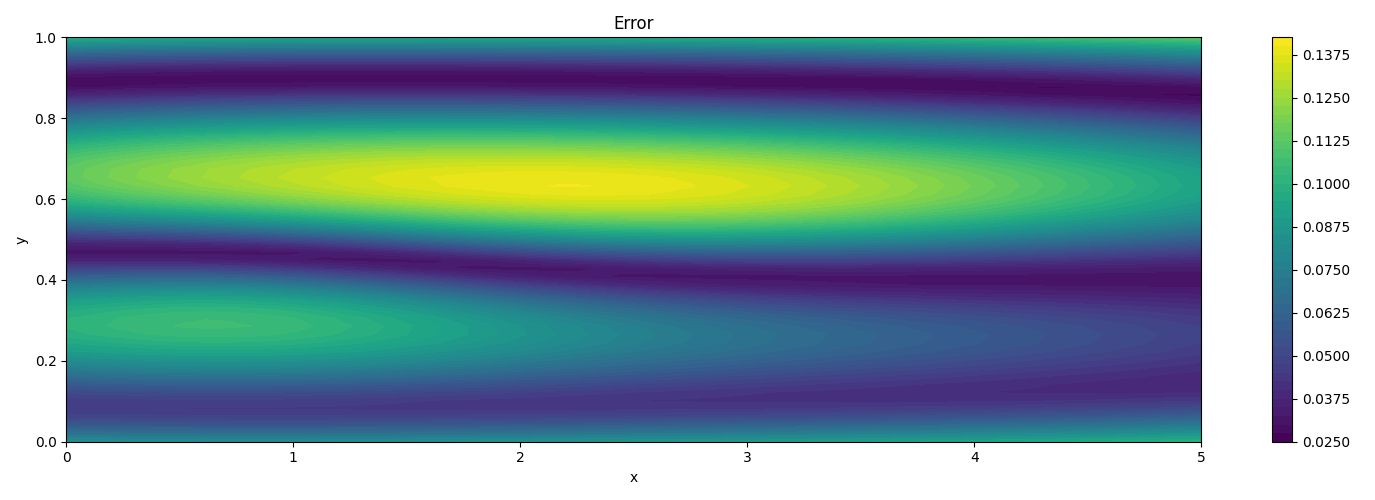
\includegraphics{data/couette_react_error_best.png}
    \caption{Результат с минимальным показателем отклонения от точного решения в процессе обучения и
    кроссвалидации модели с функцией активации REAct}
    \label{fig:couette_react_best}
\end{figure}
Также стоит отметить, что все нулевые решения соответствовали функции активации,
которая на всей области определения имеет отрицательные значения.

\begin{figure}[ht]
    \centering
    \begin{tikzpicture}
        \pgfplotstableread{
        Label   First
        NaN                     4
        Нулевое\ решение        30
        $>50\%$                 16
        $>20\%$                 94
        $<20\%$                 17
        }\datatable
        
        \begin{axis}[
            xbar stacked,
            xmin=0,
            ytick=data,
            yticklabels from table={\datatable}{Label}
            ]
            \addplot [fill=yellow] table [x=First, y expr=\coordindex] {\datatable};
        \end{axis}
    \end{tikzpicture}
    \caption{Распределение результатов кроссвалидации с функцией активации REAct}
    \label{fig:couette_react_stat}
\end{figure}

В качестве корректных параметров были отобраны те, которые соответствуют критерию
принадлежности к группе с уровнем менее 20\%. В результате, во второй этап были
включены следующие параметры:
\begin{enumerate}
    \item Конфигурации с резким переходом между слоями ($16-64-32$ и $64-16-32$) а также
    с линейным переходом ($16-32-64$ и $64-32-16$) не показали особых результатов по
    сравнению с остальными трехслойными сетями. Аналогично конфигурации
    $16-16$ и $32-32$ показали себя хуже по сравнению с $64-64$.
    \item По количеству точек внутри области значительно больше удачных
    результатов было при $100$ точек. Это поведение характеризуется 
    соотношением точек на границе и внутри области. Данное соотношение 
    показывает значимость граничных условий, что необходимо для избегания
    нулевого решения
    \item Скорость обучения влияет на то, сможет ли оптимизатор 
    выбраться из локального минимума. Лучший результат показало значение
    скорости обучения равное $10^{-3}$
    \item Среди оптимизаторов лучшие результаты показали \textbf{Adam}, \textbf{Adagrad} и
    \textbf{ASGD}, в свою очередь \textbf{Adamax} и \textbf{RSMProp} являются узкоспециализированными,
    что требует точной настройки параметров, что в данной работе не рассматривается.
\end{enumerate} 

Теперь получив более точное представление о наших параметрах можно приступить
ко второму этапу.

В представленных ниже графиках показано сравнение результатов работы нейронной сети
при различных гиперпараметрах. Такой подход позволяет детально проанализировать
влияние каждого параметра на общую эффективность модели и выявить, какие параметры
обеспечивают наилучшее качество обучения.
\begin{figure}[ht]
    \centering
    \begin{subfigure}[b]{0.4\textwidth}
        \begin{tikzpicture}
            \begin{axis}[
                ymode=log,
                % xlabel={Эпоха},
                ylabel={Медиана},
                xmin=0,
                xtick distance=4000,
                axis lines=left,
                grid=both,
                title={Нижняя граница},
                width=\textwidth
            ]
            \addplot+[mark=*, mark size=1pt, thick, red] table[x=step, y=value, col sep=comma]{data/couette_abu/loss/bc_bottom_neurons_(32, 64, 32).csv};
            \addplot+[mark=*, mark size=1pt, thick, green] table[x=step, y=value, col sep=comma]{data/couette_abu/loss/bc_bottom_neurons_(64, 32, 64).csv};
            \addplot+[mark=*, mark size=1pt, thick, blue] table[x=step, y=value, col sep=comma]{data/couette_abu/loss/bc_bottom_neurons_(64, 64).csv};
            \addplot+[mark=*, mark size=1pt, thick, orange] table[x=step, y=value, col sep=comma]{data/couette_abu/loss/bc_bottom_neurons_(128, 128).csv};
            \end{axis}
        \end{tikzpicture}
        \label{fig:bc_bottom}
    \end{subfigure}
    \hspace{0.5cm}
    \begin{subfigure}[b]{0.4\textwidth}
        \begin{tikzpicture}
            \begin{axis}[
                ymode=log,
                % xlabel={Эпоха},
                % ylabel={Медиана},
                xmin=0,
                xtick distance=4000,
                axis lines=left,
                grid=both,
                title={Верхняя граница},
                width=\textwidth
            ]
            \addplot+[mark=*, mark size=1pt, thick, red] table[x=step, y=value, col sep=comma]{data/couette_abu/loss/bc_top_neurons_(32, 64, 32).csv};
            \addplot+[mark=*, mark size=1pt, thick, green] table[x=step, y=value, col sep=comma]{data/couette_abu/loss/bc_top_neurons_(64, 32, 64).csv};
            \addplot+[mark=*, mark size=1pt, thick, blue] table[x=step, y=value, col sep=comma]{data/couette_abu/loss/bc_top_neurons_(64, 64).csv};
            \addplot+[mark=*, mark size=1pt, thick, orange] table[x=step, y=value, col sep=comma]{data/couette_abu/loss/bc_top_neurons_(128, 128).csv};
            \end{axis}
        \end{tikzpicture}
        \label{fig:bc_top}
    \end{subfigure}
    \vspace{0.05cm}
    \begin{subfigure}[b]{0.4\textwidth}
        \begin{tikzpicture}
            \begin{axis}[
                ymode=log,
                xlabel={Эпоха},
                ylabel={Медиана},
                xmin=0,
                xtick distance=4000,
                axis lines=left,
                grid=both,
                title={Левая граница},
                width=\textwidth
            ]
            \addplot+[mark=*, mark size=1pt, thick, red] table[x=step, y=value, col sep=comma]{data/couette_abu/loss/bc_left_neurons_(32, 64, 32).csv};
            \addplot+[mark=*, mark size=1pt, thick, green] table[x=step, y=value, col sep=comma]{data/couette_abu/loss/bc_left_neurons_(64, 32, 64).csv};
            \addplot+[mark=*, mark size=1pt, thick, blue] table[x=step, y=value, col sep=comma]{data/couette_abu/loss/bc_left_neurons_(64, 64).csv};
            \addplot+[mark=*, mark size=1pt, thick, orange] table[x=step, y=value, col sep=comma]{data/couette_abu/loss/bc_left_neurons_(128, 128).csv};
            \end{axis}
        \end{tikzpicture}
        \label{fig:bc_left}
    \end{subfigure}
    \hspace{0.5cm}
    \begin{subfigure}[b]{0.4\textwidth}
        \begin{tikzpicture}
            \begin{axis}[
                ymode=log,
                xlabel={Эпоха},
                % ylabel={Медиана},
                xmin=0,
                xtick distance=4000,
                axis lines=left,
                grid=both,
                title={Правая граница},
                width=\textwidth
            ]
            \addplot+[mark=*, mark size=1pt, thick, red] table[x=step, y=value, col sep=comma]{data/couette_abu/loss/bc_right_neurons_(32, 64, 32).csv};
            \addplot+[mark=*, mark size=1pt, thick, green] table[x=step, y=value, col sep=comma]{data/couette_abu/loss/bc_right_neurons_(64, 32, 64).csv};
            \addplot+[mark=*, mark size=1pt, thick, blue] table[x=step, y=value, col sep=comma]{data/couette_abu/loss/bc_right_neurons_(64, 64).csv};
            \addplot+[mark=*, mark size=1pt, thick, orange] table[x=step, y=value, col sep=comma]{data/couette_abu/loss/bc_right_neurons_(128, 128).csv};
            \end{axis}
        \end{tikzpicture}
        \label{fig:bc_right}
    \end{subfigure}
    \caption{Зависимость медианы функции потерь на каждой эпохе при разной конфигурации нейронной сети}
    \label{fig:bc_loss_neurons}
\end{figure}

%%%%%%%%%%%%%%%%%%%%%%%%%%%%%%%%%%%%%%%%%%%%%%%%%%%%%%%%%%%%%%%%%%%%%%%%%%%%%%

\begin{figure}[htbp]
    \centering
    \begin{subfigure}[b]{0.4\textwidth}
        \begin{tikzpicture}
            \begin{axis}[
                ymode=log,
                ymin=1e-4, ymax=1e-2,
                xlabel={Эпоха},
                ylabel={Медиана},
                xmin=0,
                xtick distance=4000,
                axis lines=left,
                grid=both,
                title={Уравнение для $v_x$},
                width=\textwidth
            ]
            \addplot+[mark=*, mark size=1pt, thick, red] table[x=step, y=value, col sep=comma]{data/couette_abu/loss/pde_momentum_x_neurons_(32, 64, 32).csv};
            \addplot+[mark=*, mark size=1pt, thick, green] table[x=step, y=value, col sep=comma]{data/couette_abu/loss/pde_momentum_x_neurons_(64, 32, 64).csv};
            \addplot+[mark=*, mark size=1pt, thick, blue] table[x=step, y=value, col sep=comma]{data/couette_abu/loss/pde_momentum_x_neurons_(64, 64).csv};
            \addplot+[mark=*, mark size=1pt, thick, orange] table[x=step, y=value, col sep=comma]{data/couette_abu/loss/pde_momentum_x_neurons_(128, 128).csv};
            \end{axis}
        \end{tikzpicture}
    \end{subfigure}
    \hspace{0.5cm}
    \begin{subfigure}[b]{0.4\textwidth}
        \begin{tikzpicture}
            \begin{axis}[
                ymode=log,
                ymin=1e-4, ymax=1e-2,
                xlabel={Эпоха},
                % ylabel={Медиана},
                xmin=0,
                xtick distance=4000,
                axis lines=left,
                grid=both,
                title={Уравнение для $v_y$},
                width=\textwidth
            ]
            \addplot+[mark=*, mark size=1pt, thick, red] table[x=step, y=value, col sep=comma]{data/couette_abu/loss/pde_momentum_y_neurons_(32, 64, 32).csv};
            \addplot+[mark=*, mark size=1pt, thick, green] table[x=step, y=value, col sep=comma]{data/couette_abu/loss/pde_momentum_y_neurons_(64, 32, 64).csv};
            \addplot+[mark=*, mark size=1pt, thick, blue] table[x=step, y=value, col sep=comma]{data/couette_abu/loss/pde_momentum_y_neurons_(64, 64).csv};
            \addplot+[mark=*, mark size=1pt, thick, orange] table[x=step, y=value, col sep=comma]{data/couette_abu/loss/pde_momentum_y_neurons_(128, 128).csv};
            \end{axis}
        \end{tikzpicture}
    \end{subfigure}
    \begin{subfigure}[b]{0.7\textwidth}
        \begin{tikzpicture}
            \begin{axis}[
                ymode=log,
                ymin=1e-4, ymax=1e-2,
                xlabel={Эпоха},
                ylabel={Медиана},
                xmin=0,
                xtick distance=1000,
                axis lines=left,
                grid=both,
                title={Уравнение непрерывности},
                width=\textwidth
            ]
            \addplot+[mark=*, mark size=1pt, thick, red] table[x=step, y=value, col sep=comma]{data/couette_abu/loss/pde_continuity_neurons_(32, 64, 32).csv};
            % \addlegendentry{(32, 64, 32)}
            \addplot+[mark=*, mark size=1pt, thick, green] table[x=step, y=value, col sep=comma]{data/couette_abu/loss/pde_continuity_neurons_(64, 32, 64).csv};
            % \addlegendentry{(64, 32, 64)}
            \addplot+[mark=*, mark size=1pt, thick, blue] table[x=step, y=value, col sep=comma]{data/couette_abu/loss/pde_continuity_neurons_(64, 64).csv};
            % \addlegendentry{(64, 64)}
            \addplot+[mark=*, mark size=1pt, thick, orange] table[x=step, y=value, col sep=comma]{data/couette_abu/loss/pde_continuity_neurons_(128, 128).csv};
            % \addlegendentry{(128, 128)}
        \end{axis}
        \end{tikzpicture}
    \end{subfigure}
    \caption{Функция потерь для уравнений Навье-Стокса \eqref{eq:navier_stockes} при разной конфигурации нейронной сети}
    \label{fig:pde_loss_neurons}
\end{figure}

%%%%%%%%%%%%%%%%%%%%%%%%%%%%%%%%%%%%%%%%%%%%%%%%%%%%%%%%%%%%%%%%%%

\begin{figure}[htbp]
    \centering
    \begin{tikzpicture}
        \begin{axis}[
            width=0.8\textwidth,
            ymode=log,
            xlabel={Эпоха},
            ylabel={Медиана},
            xmin=0,
            xtick distance=1000,
            axis lines=left,
            grid=both,
        ]
            \addplot+[mark=*, mark size=1pt, thick, red] table[x=step, y=value, col sep=comma]{data/couette_abu/loss/total_loss_neurons_(32, 64, 32).csv};
            \addlegendentry{(32, 64, 32)}
            \addplot+[mark=*, mark size=1pt, thick, green] table[x=step, y=value, col sep=comma]{data/couette_abu/loss/total_loss_neurons_(64, 32, 64).csv};
            \addlegendentry{(64, 32, 64)}
            \addplot+[mark=*, mark size=1pt, thick, blue] table[x=step, y=value, col sep=comma]{data/couette_abu/loss/total_loss_neurons_(64, 64).csv};
            \addlegendentry{(64, 64)}
            \addplot+[mark=*, mark size=1pt, thick, orange] table[x=step, y=value, col sep=comma]{data/couette_abu/loss/total_loss_neurons_(128, 128).csv};
            \addlegendentry{(128, 128)}
        \end{axis}
    \end{tikzpicture}
    \caption{Итоговая функция потерь при разной конфигурации нейронной сети}
    \label{fig:total_loss_neurons}
\end{figure}
\section{Зависимость от оптимизатора}

С точки зрения оптимизатора никаких ограничений на поведение
модели нет. От выбора оптимизатора зависит на сколько сложно
модели будет выбраться из локального минимума и приблизиться
к глобальному.

Рассмотрим верхнюю границу (рис \ref{fig:bc_top_optimizer}).
Исходя из графика, при использовании оптимизатора ASGD
функция потерь в среднем стремится к $~0.25$. При такой 
функции потерь максимальное отклонение от точного решения
может достигать $50\%$, если не учитывать полностью
нулевые решения. Сам по себе ASGD является мощным оптимизатором,
но требует тонкой настройки своих параметров, поэтому он
показывает худший результат в данной задаче.

Похожая ситуация с Adagrad оптимизатором, без качественной
настройки параметров скорость обучения адаптивно уменьшается
и оптимизатор застывает в локальном минимуме. Вероятнее всего
при большем числе эпох Adagrad сможет догнать Adam, но нас
данный вариант не устраивает.

Оптимизатор Adam показывает лучший результат. Данный оптимизатор
включает в себя преймущества двух предыдущих и является универсальным,
поэтому не требует такой же точной настройки параметров.

\begin{figure}[ht]
    \centering
    \begin{subfigure}[b]{0.4\textwidth}
        \begin{tikzpicture}[scale=0.85]
            \begin{axis}[
                ymode=log,
                legend style={font=\tiny},
                xmin=0,
                xtick distance=4000,
                axis lines=left,
                grid=both
            ]            
                \addplot+[mark=*, mark size=1pt, thick, red] table[x=step, y=value, col sep=comma]{data/couette_abu/loss/bc_bottom_optimizer_1.csv};
                \addlegendentry{Adam}
                \addplot+[mark=*, mark size=1pt, thick, green] table[x=step, y=value, col sep=comma]{data/couette_abu/loss/bc_bottom_optimizer_2.csv};
                \addlegendentry{Adagrad}
                \addplot+[mark=*, mark size=1pt, thick, blue] table[x=step, y=value, col sep=comma]{data/couette_abu/loss/bc_bottom_optimizer_4.csv};
                \addlegendentry{ASGD}
            \end{axis}
        \end{tikzpicture}
        \caption{Нижняя граница}
        \label{fig:bc_bottom_optimizer}
    \end{subfigure}
    \hspace{0.5cm}
    \begin{subfigure}[b]{0.4\textwidth}
        \begin{tikzpicture}[scale=0.85]
            \begin{axis}[
                ymode=log,
                legend style={font=\tiny},
                xmin=0,
                xtick distance=4000,
                axis lines=left,
                grid=both
            ]
                \addplot+[mark=*, mark size=1pt, thick, red] table[x=step, y=value, col sep=comma]{data/couette_abu/loss/bc_top_optimizer_1.csv};
                \addlegendentry{Adam}
                \addplot+[mark=*, mark size=1pt, thick, green] table[x=step, y=value, col sep=comma]{data/couette_abu/loss/bc_top_optimizer_2.csv};
                \addlegendentry{Adagrad}
                \addplot+[mark=*, mark size=1pt, thick, blue] table[x=step, y=value, col sep=comma]{data/couette_abu/loss/bc_top_optimizer_4.csv};
                \addlegendentry{ASGD}
            \end{axis}
        \end{tikzpicture}
        \caption{Верхняя граница}
        \label{fig:bc_top_optimizer}
    \end{subfigure}
    \begin{subfigure}[b]{0.4\textwidth}
        \begin{tikzpicture}[scale=0.85]
            \begin{axis}[
                ymode=log,
                legend style={font=\tiny},
                xmin=0,
                xtick distance=4000,
                axis lines=left,
                grid=both
            ]
                \addplot+[mark=*, mark size=1pt, thick, red] table[x=step, y=value, col sep=comma]{data/couette_abu/loss/bc_left_optimizer_1.csv};
                \addlegendentry{Adam}
                \addplot+[mark=*, mark size=1pt, thick, green] table[x=step, y=value, col sep=comma]{data/couette_abu/loss/bc_left_optimizer_2.csv};
                \addlegendentry{Adagrad}
                \addplot+[mark=*, mark size=1pt, thick, blue] table[x=step, y=value, col sep=comma]{data/couette_abu/loss/bc_left_optimizer_4.csv};
                \addlegendentry{ASGD}
            \end{axis}
        \end{tikzpicture}
        \caption{Левая граница}
        \label{fig:bc_left_optimizer}
    \end{subfigure}
    \hspace{0.5cm}
    \begin{subfigure}[b]{0.4\textwidth}
        \begin{tikzpicture}[scale=0.85]
            \begin{axis}[
                ymode=log,
                legend style={font=\tiny},
                xmin=0,
                xtick distance=4000,
                axis lines=left,
                grid=both
            ]
                \addplot+[mark=*, mark size=1pt, thick, red] table[x=step, y=value, col sep=comma]{data/couette_abu/loss/bc_right_optimizer_1.csv};
                \addlegendentry{Adam}
                \addplot+[mark=*, mark size=1pt, thick, green] table[x=step, y=value, col sep=comma]{data/couette_abu/loss/bc_right_optimizer_2.csv};
                \addlegendentry{Adagrad}
                \addplot+[mark=*, mark size=1pt, thick, blue] table[x=step, y=value, col sep=comma]{data/couette_abu/loss/bc_right_optimizer_4.csv};
                \addlegendentry{ASGD}
            \end{axis}
        \end{tikzpicture}
        \caption{Правая граница}
        \label{fig:bc_right_optimizer}
    \end{subfigure}
    \caption{Зависимость медианы функции потерь на каждой эпохе при разных оптимизаторах}
    \label{fig:bc_loss_optimizer}
\end{figure}

Аналогичное поведение оптимизаторов можно заметить на графике для нижней
границы (рис. \ref{fig:bc_bottom_optimizer}). На графиках левой
(рис. \ref{fig:bc_left_optimizer}) и правой (рис. \ref{fig:bc_right_optimizer})
границах можно заметить смещение оптимизатора ASGD ближе к Adagrad, что может
свидетельствовать о преобладающем нулевом решении.

%%%%%%%%%%%%%%%%%%%%%%%%%%%%%%%%%%%%%%%%%%%%%%%%%%%%%%%%%%%%%%%%%%%%%%%%%%%%%%

\begin{figure}[htbp]
    \centering
    \begin{subfigure}[b]{0.4\textwidth}
        \centering
        \begin{tikzpicture}[scale=0.85]
            \begin{axis}[
                ymode=log,
                ymax=1e-2,
                legend style={font=\tiny},
                xmin=0,
                xtick distance=4000,
                axis lines=left,
                grid=both
            ]
                \addplot+[mark=*, mark size=1pt, thick, red] table[x=step, y=value, col sep=comma]{data/couette_abu/loss/pde_momentum_x_optimizer_1.csv};
                \addlegendentry{Adam}
                \addplot+[mark=*, mark size=1pt, thick, green] table[x=step, y=value, col sep=comma]{data/couette_abu/loss/pde_momentum_x_optimizer_2.csv};
                \addlegendentry{Adagrad}
                \addplot+[mark=*, mark size=1pt, thick, blue] table[x=step, y=value, col sep=comma]{data/couette_abu/loss/pde_momentum_x_optimizer_4.csv};
                \addlegendentry{ASGD}
            \end{axis}
        \end{tikzpicture}
        \caption{Уравнение для $u_x$}
        \label{fig:pde_ux_optimizer}
    \end{subfigure}
    \hspace{0.5cm}
    \begin{subfigure}[b]{0.4\textwidth}
        \centering
        \begin{tikzpicture}[scale=0.85]
            \begin{axis}[
                ymode=log,
                ymax=1e-2,
                legend style={font=\tiny},
                xmin=0,
                xtick distance=4000,
                axis lines=left,
                grid=both
            ]
                \addplot+[mark=*, mark size=1pt, thick, red] table[x=step, y=value, col sep=comma]{data/couette_abu/loss/pde_momentum_y_optimizer_1.csv};
                \addlegendentry{Adam}
                \addplot+[mark=*, mark size=1pt, thick, green] table[x=step, y=value, col sep=comma]{data/couette_abu/loss/pde_momentum_y_optimizer_2.csv};
                \addlegendentry{Adagrad}
                \addplot+[mark=*, mark size=1pt, thick, blue] table[x=step, y=value, col sep=comma]{data/couette_abu/loss/pde_momentum_y_optimizer_4.csv};
                \addlegendentry{ASGD}
            \end{axis}
        \end{tikzpicture}
        \caption{Уравнение для $u_y$}
        \label{fig:pde_uy_optimizer}
    \end{subfigure}
    \begin{subfigure}[b]{0.7\textwidth}
        \centering
        \begin{tikzpicture}
            \begin{axis}[
                ymode=log,
                ymax=1e-2,
                legend style={font=\small},
                xmin=0,
                xtick distance=1000,
                axis lines=left,
                grid=both,
                width=\textwidth
            ]
                \addplot+[mark=*, mark size=1pt, thick, red] table[x=step, y=value, col sep=comma]{data/couette_abu/loss/pde_continuity_optimizer_1.csv};
                \addlegendentry{Adam}
                \addplot+[mark=*, mark size=1pt, thick, green] table[x=step, y=value, col sep=comma]{data/couette_abu/loss/pde_continuity_optimizer_2.csv};
                \addlegendentry{Adagrad}
                \addplot+[mark=*, mark size=1pt, thick, blue] table[x=step, y=value, col sep=comma]{data/couette_abu/loss/pde_continuity_optimizer_4.csv};
                \addlegendentry{ASGD}
            \end{axis}
        \end{tikzpicture}
        \caption{Уравнение непрерывности}
        \label{fig:pde_continuity_optimizer}
    \end{subfigure}
    \caption{Функция потерь для уравнений Навье-Стокса \eqref{eq:navier_stockes} при разных оптимизаторах}
    \label{fig:pde_loss_optimizer}
\end{figure}

Для уравнений Навье-Стокса можно заметить рост функции потерь для оптимизатора
ASGD (рис. \ref{fig:pde_ux_optimizer} и \ref{fig:pde_continuity_optimizer}).
Таким образом происходит процесс поиска глобального минимума. Дело в том,
что функция потерь для верхней границы много больше, чем для уравнений Навье-Стокса
($10^{-0.8}$ против $10^{-2.9}$). Оптимизатор пытается выбраться из локального 
минимума, где решение стремится к нулевому в силу своей корректности с точки
зрения уравнений Навье-Стокса. Что касательно уравнения для скорости $u_y$
(рис. \ref{fig:pde_uy_optimizer}), график оптимизатора ASGD остается
практически неизменным, что опять же соответствует нулевому решению.
Остальные оптимизаторы имеют поведение схожее с поведением на границах.


%%%%%%%%%%%%%%%%%%%%%%%%%%%%%%%%%%%%%%%%%%%%%%%%%%%%%%%%%%%%%%%%%%

\begin{figure}[htbp]
    \centering
    \begin{tikzpicture}
        \begin{axis}[
            width=0.8\textwidth,
            ymode=log,
            xmin=0,
            xtick distance=1000,
            axis lines=left,
            grid=both,
        ]
            \addplot+[mark=*, mark size=1pt, thick, red] table[x=step, y=value, col sep=comma]{data/couette_abu/loss/total_loss_optimizer_1.csv};
            \addlegendentry{Adam}
            \addplot+[mark=*, mark size=1pt, thick, green] table[x=step, y=value, col sep=comma]{data/couette_abu/loss/total_loss_optimizer_2.csv};
            \addlegendentry{Adagrad}
            \addplot+[mark=*, mark size=1pt, thick, blue] table[x=step, y=value, col sep=comma]{data/couette_abu/loss/total_loss_optimizer_4.csv};
            \addlegendentry{ASGD}
        \end{axis}
    \end{tikzpicture}
    \caption{Итоговая функция потерь при разных оптимизаторах}
    \label{fig:total_loss_optimizer}
\end{figure}

Итого на суммарной функции потерь (рис. \ref{fig:total_loss_optimizer}),
оптимизатор Adam имеет наименьшую функцию потерь.
\section{Зависимость от фукции активации ABU}

В первую очередь функция активация играет основополагающую роль для
детерминирования поведения внутри исследуемой области. Это связано с тем,
что уравнения Навье-Стокса имеют сложную структуру и если поставленная
задача имеет не нулевое решение, то нахождение верного решения внутри
домена в основном зависит от функции активации.

Как ранее упоминалось, ABU является взвешенной суммой элементарных функций
активации \eqref{eq:abu_custom}. Рассмотрим влияние каждого слагаемого на
функцию потерь.
\subsection{Квадратичная функция}
Нужно понимать, что введение нелинейности в решение не всегда помогает
найти более точное решение. Наблюдая за функцией потерь
(рис. \ref{fig:pde_loss_scale_quadratic}) можно заметить, что для уравнения
непрерывности (рис. \ref{fig:pde_continuity_scale_quadratic}) и уравнения
компоненты $u_x$ (рис. \ref{fig:pde_ux_scale_quadratic}) поведение 
остается одинаковым, однако для компоненты $u_y$ (рис. \ref{fig:pde_uy_scale_quadratic})
доминирует $\beta_2 = 0.0$.
% Как упоминалось ранее, точным решением
% для $u_y$ является нулевое решение на всей решаемой области, что является,
% пожалуй, самым сложным с точки зрения нейронной сети. Дело в том, 


\begin{figure}[H]
    \centering
    \begin{subfigure}[b]{0.4\textwidth}
        \centering
        \begin{tikzpicture}[scale=0.85]
            \begin{axis}[
                ymode=log,
                ymax=1e-2,
                legend style={font=\tiny},
                xmin=0,
                xtick distance=4000,
                axis lines=left,
                grid=both
            ]
                \addplot+[mark=*, mark size=1pt, thick, red] table[x=step, y=value, col sep=comma]{data/couette_abu/loss/pde_momentum_x_scale_quadratic_0.0.csv};
                \addlegendentry{$0.0$}
                \addplot+[mark=*, mark size=1pt, thick, green] table[x=step, y=value, col sep=comma]{data/couette_abu/loss/pde_momentum_x_scale_quadratic_1.0.csv};
                \addlegendentry{$1.0$}
            \end{axis}
        \end{tikzpicture}
        \caption{Уравнение для $u_x$}
        \label{fig:pde_ux_scale_quadratic}
    \end{subfigure}
    \hspace{0.5cm}
    \begin{subfigure}[b]{0.4\textwidth}
        \centering
        \begin{tikzpicture}[scale=0.85]
            \begin{axis}[
                ymode=log,
                ymax=1e-2,
                legend style={font=\tiny},
                xmin=0,
                xtick distance=4000,
                axis lines=left,
                grid=both
            ]
                \addplot+[mark=*, mark size=1pt, thick, red] table[x=step, y=value, col sep=comma]{data/couette_abu/loss/pde_momentum_y_scale_quadratic_0.0.csv};
                \addlegendentry{$0.0$}
                \addplot+[mark=*, mark size=1pt, thick, green] table[x=step, y=value, col sep=comma]{data/couette_abu/loss/pde_momentum_y_scale_quadratic_1.0.csv};
                \addlegendentry{$1.0$}
            \end{axis}
        \end{tikzpicture}
        \caption{Уравнение для $u_y$}
        \label{fig:pde_uy_scale_quadratic}
    \end{subfigure}
    \begin{subfigure}[b]{0.7\textwidth}
        \centering
        \begin{tikzpicture}[scale=0.85]
            \begin{axis}[
                ymode=log,
                ymax=1e-2,
                legend style={font=\tiny},
                xmin=0,
                xtick distance=2000,
                axis lines=left,
                grid=both
            ]
                \addplot+[mark=*, mark size=1pt, thick, red] table[x=step, y=value, col sep=comma]{data/couette_abu/loss/pde_continuity_scale_quadratic_0.0.csv};
                \addlegendentry{$0.0$}
                \addplot+[mark=*, mark size=1pt, thick, green] table[x=step, y=value, col sep=comma]{data/couette_abu/loss/pde_continuity_scale_quadratic_1.0.csv};
                \addlegendentry{$1.0$}
            \end{axis}
        \end{tikzpicture}
        \caption{Уравнение непрерывности}
        \label{fig:pde_continuity_scale_quadratic}
    \end{subfigure}
    \caption{Функция потерь для уравнений Навье-Стокса \eqref{eq:navier_stockes} при разных коэффициентов для функции активации Quadratic}
    \label{fig:pde_loss_scale_quadratic}
\end{figure}


%%%%%%%%%%%%%%%%%%%%%%%%%%%%%%%%%%%%%%%%%%%%%%%%%%%%%%%%%%%%%%%%%%
В целом данный вывод подтверждается и на графике общей функции потерь
(рис. \ref{fig:pde_loss_scale_quadratic}). Это объясняется линейностью
решения задачи, где отсутствует квадратичная нелинейность.
\begin{figure}[H]
    \centering
    \begin{tikzpicture}
        \begin{axis}[
            width=0.5\textwidth,
            ymode=log,
            xmin=0,
            xtick distance=2000,
            axis lines=left,
            grid=both,
        ]
            \addplot+[mark=*, mark size=1pt, thick, red] table[x=step, y=value, col sep=comma]{data/couette_abu/loss/total_loss_scale_quadratic_0.0.csv};
            \addlegendentry{$0.0$}
            \addplot+[mark=*, mark size=1pt, thick, green] table[x=step, y=value, col sep=comma]{data/couette_abu/loss/total_loss_scale_quadratic_1.0.csv};
            \addlegendentry{$1.0$}
        \end{axis}
    \end{tikzpicture}
    \caption{Итоговая функция потерь при разных коэффициентов для функции активации Quadratic}
    \label{fig:total_loss_scale_quadratic}
\end{figure}

\subsection{Softplus функция}

\begin{figure}[H]
    \centering
    \begin{subfigure}[b]{0.4\textwidth}
        \centering
        \begin{tikzpicture}[scale=0.85]
            \begin{axis}[
                ymode=log,
                ymax=1e-2,
                legend style={font=\tiny},
                xmin=0,
                xtick distance=4000,
                axis lines=left,
                grid=both
            ]
                \addplot+[mark=*, mark size=1pt, thick, red] table[x=step, y=value, col sep=comma]{data/couette_abu/loss/pde_momentum_x_scale_softplus_0.0.csv};
                \addlegendentry{$0.0$}
                \addplot+[mark=*, mark size=1pt, thick, green] table[x=step, y=value, col sep=comma]{data/couette_abu/loss/pde_momentum_x_scale_softplus_1.0.csv};
                \addlegendentry{$1.0$}
            \end{axis}
        \end{tikzpicture}
        \caption{Уравнение для $u_x$}
        \label{fig:pde_ux_scale_softplus}
    \end{subfigure}
    \hspace{0.5cm}
    \begin{subfigure}[b]{0.4\textwidth}
        \centering
        \begin{tikzpicture}[scale=0.85]
            \begin{axis}[
                ymode=log,
                ymax=1e-2,
                legend style={font=\tiny},
                xmin=0,
                xtick distance=4000,
                axis lines=left,
                grid=both
            ]
                \addplot+[mark=*, mark size=1pt, thick, red] table[x=step, y=value, col sep=comma]{data/couette_abu/loss/pde_momentum_y_scale_softplus_0.0.csv};
                \addlegendentry{$0.0$}
                \addplot+[mark=*, mark size=1pt, thick, green] table[x=step, y=value, col sep=comma]{data/couette_abu/loss/pde_momentum_y_scale_softplus_1.0.csv};
                \addlegendentry{$1.0$}
            \end{axis}
        \end{tikzpicture}
        \caption{Уравнение для $u_y$}
        \label{fig:pde_uy_scale_softplus}
    \end{subfigure}
    \begin{subfigure}[b]{0.7\textwidth}
        \centering
        \begin{tikzpicture}[scale=0.85]
            \begin{axis}[
                ymode=log,
                ymax=1e-2,
                legend style={font=\tiny},
                xmin=0,
                xtick distance=2000,
                axis lines=left,
                grid=both
            ]
                \addplot+[mark=*, mark size=1pt, thick, red] table[x=step, y=value, col sep=comma]{data/couette_abu/loss/pde_continuity_scale_softplus_0.0.csv};
                \addlegendentry{$0.0$}
                \addplot+[mark=*, mark size=1pt, thick, green] table[x=step, y=value, col sep=comma]{data/couette_abu/loss/pde_continuity_scale_softplus_1.0.csv};
                \addlegendentry{$1.0$}
            \end{axis}
        \end{tikzpicture}
        \caption{Уравнение непрерывности}
        \label{fig:pde_continuity_scale_softplus}
    \end{subfigure}
    \caption{Функция потерь для уравнений Навье-Стокса \eqref{eq:navier_stockes} при разных коэффициентов для функции активации Softplus}
    \label{fig:pde_loss_scale_softplus}
\end{figure}

Данная функция пусть и не линейная, но данная нелинейность проявляется в 
окрестностях нуля, что позволяет посчитать аналитически значение ее производных.
На остальном же промежутке можно ее считать линейной, что вводит линейность в наше решение.
Как видно из графиков для уравнений Навье-Стокса (рис. \ref{fig:pde_loss_scale_softplus}),
при $\beta_1 = 0$ получаемый результат незначительно лучше. 


%%%%%%%%%%%%%%%%%%%%%%%%%%%%%%%%%%%%%%%%%%%%%%%%%%%%%%%%%%%%%%%%%%
Однако в силу потерь на границах, на графике общей функции потерь видим обратное:
при $\beta_1 = 1$ результат значительно лучше
(рис. \ref{fig:total_loss_scale_softplus}).

\begin{figure}[H]
    \centering
    \begin{tikzpicture}
        \begin{axis}[
            width=0.6\textwidth,
            ymode=log,
            xmin=0,
            xtick distance=2000,
            axis lines=left,
            grid=both,
        ]
            \addplot+[mark=*, mark size=1pt, thick, red] table[x=step, y=value, col sep=comma]{data/couette_abu/loss/total_loss_scale_softplus_0.0.csv};
            \addlegendentry{$0.0$}
            \addplot+[mark=*, mark size=1pt, thick, green] table[x=step, y=value, col sep=comma]{data/couette_abu/loss/total_loss_scale_softplus_1.0.csv};
            \addlegendentry{$1.0$}
        \end{axis}
    \end{tikzpicture}
    \caption{Итоговая функция потерь при разных коэффициентов для функции активации Softplus}
    \label{fig:total_loss_scale_softplus}
\end{figure}

% \subsection{SiLU функция}
\subsection{SiLU и Tanh функция}
Аналогичный результат присутствует и для функций активации SiLU и Tanh. Одной
из причин такого поведения является маленькая выборка коэффициентов $\beta_i$.
Второй причиной является присутствие шума в виде ранее отсеяных оптимизаторов
и конфигурации слоев. Для более сложных задач следует проводить повторную
кроссвалидацию каждый раз после фильтрации кросспараметров, добавляя больше
параметров для качественного результата.
% \begin{figure}[H]
%     \centering
%     \begin{subfigure}[b]{0.4\textwidth}
%         \centering
%         \begin{tikzpicture}[scale=0.85]
%             \begin{axis}[
%                 ymode=log,
%                 ymax=1e-2,
%                 legend style={font=\tiny},
%                 xmin=0,
%                 xtick distance=4000,
%                 axis lines=left,
%                 grid=both
%             ]
%                 \addplot+[mark=*, mark size=1pt, thick, red] table[x=step, y=value, col sep=comma]{data/couette_abu/loss/pde_momentum_x_scale_swish_0.0.csv};
%                 \addlegendentry{$0.0$}
%                 \addplot+[mark=*, mark size=1pt, thick, green] table[x=step, y=value, col sep=comma]{data/couette_abu/loss/pde_momentum_x_scale_swish_1.0.csv};
%                 \addlegendentry{$1.0$}
%             \end{axis}
%         \end{tikzpicture}
%         \caption{Уравнение для $u_x$}
%         \label{fig:pde_ux_scale_swish}
%     \end{subfigure}
%     \hspace{0.5cm}
%     \begin{subfigure}[b]{0.4\textwidth}
%         \centering
%         \begin{tikzpicture}[scale=0.85]
%             \begin{axis}[
%                 ymode=log,
%                 ymax=1e-2,
%                 legend style={font=\tiny},
%                 xmin=0,
%                 xtick distance=4000,
%                 axis lines=left,
%                 grid=both
%             ]
%                 \addplot+[mark=*, mark size=1pt, thick, red] table[x=step, y=value, col sep=comma]{data/couette_abu/loss/pde_momentum_y_scale_swish_0.0.csv};
%                 \addlegendentry{$0.0$}
%                 \addplot+[mark=*, mark size=1pt, thick, green] table[x=step, y=value, col sep=comma]{data/couette_abu/loss/pde_momentum_y_scale_swish_1.0.csv};
%                 \addlegendentry{$1.0$}
%             \end{axis}
%         \end{tikzpicture}
%         \caption{Уравнение для $u_y$}
%         \label{fig:pde_uy_scale_swish}
%     \end{subfigure}
%     \begin{subfigure}[b]{0.7\textwidth}
%         \centering
%         \begin{tikzpicture}[scale=0.85]
%             \begin{axis}[
%                 ymode=log,
%                 ymax=1e-2,
%                 legend style={font=\tiny},
%                 xmin=0,
%                 xtick distance=2000,
%                 axis lines=left,
%                 grid=both
%             ]
%                 \addplot+[mark=*, mark size=1pt, thick, red] table[x=step, y=value, col sep=comma]{data/couette_abu/loss/pde_continuity_scale_swish_0.0.csv};
%                 \addlegendentry{$0.0$}
%                 \addplot+[mark=*, mark size=1pt, thick, green] table[x=step, y=value, col sep=comma]{data/couette_abu/loss/pde_continuity_scale_swish_1.0.csv};
%                 \addlegendentry{$1.0$}
%             \end{axis}
%         \end{tikzpicture}
%         \caption{Уравнение непрерывности}
%         \label{fig:pde_continuity_scale_swish}
%     \end{subfigure}
%     \caption{Функция потерь для уравнений Навье-Стокса \eqref{eq:navier_stockes} при разных коэффициентов для функции активации SiLU}
%     \label{fig:pde_loss_scale_swish}
% \end{figure}

% %%%%%%%%%%%%%%%%%%%%%%%%%%%%%%%%%%%%%%%%%%%%%%%%%%%%%%%%%%%%%%%%%%

% \begin{figure}[H]
%     \centering
%     \begin{tikzpicture}
%         \begin{axis}[
%             width=0.6\textwidth,
%             ymode=log,
%             xmin=0,
%             xtick distance=2000,
%             axis lines=left,
%             grid=both,
%         ]
%             \addplot+[mark=*, mark size=1pt, thick, red] table[x=step, y=value, col sep=comma]{data/couette_abu/loss/total_loss_scale_swish_0.0.csv};
%             \addlegendentry{$0.0$}
%             \addplot+[mark=*, mark size=1pt, thick, green] table[x=step, y=value, col sep=comma]{data/couette_abu/loss/total_loss_scale_swish_1.0.csv};
%             \addlegendentry{$1.0$}
%         \end{axis}
%     \end{tikzpicture}
%     \caption{Итоговая функция потерь при разных коэффициентов для функции активации SiLU}
%     \label{fig:total_loss_scale_swish}
% \end{figure}


% \subsection{Tanh функция}

% \begin{figure}[H]
%     \centering
%     \begin{subfigure}[b]{0.4\textwidth}
%         \centering
%         \begin{tikzpicture}[scale=0.85]
%             \begin{axis}[
%                 ymode=log,
%                 ymax=1e-2,
%                 legend style={font=\tiny},
%                 xmin=0,
%                 xtick distance=4000,
%                 axis lines=left,
%                 grid=both
%             ]
%                 \addplot+[mark=*, mark size=1pt, thick, red] table[x=step, y=value, col sep=comma]{data/couette_abu/loss/pde_momentum_x_scale_tanh_0.0.csv};
%                 \addlegendentry{$0.0$}
%                 \addplot+[mark=*, mark size=1pt, thick, green] table[x=step, y=value, col sep=comma]{data/couette_abu/loss/pde_momentum_x_scale_tanh_1.0.csv};
%                 \addlegendentry{$1.0$}
%             \end{axis}
%         \end{tikzpicture}
%         \caption{Уравнение для $u_x$}
%         \label{fig:pde_ux_scale_tanh}
%     \end{subfigure}
%     \hspace{0.5cm}
%     \begin{subfigure}[b]{0.4\textwidth}
%         \centering
%         \begin{tikzpicture}[scale=0.85]
%             \begin{axis}[
%                 ymode=log,
%                 ymax=1e-2,
%                 legend style={font=\tiny},
%                 xmin=0,
%                 xtick distance=4000,
%                 axis lines=left,
%                 grid=both
%             ]
%                 \addplot+[mark=*, mark size=1pt, thick, red] table[x=step, y=value, col sep=comma]{data/couette_abu/loss/pde_momentum_y_scale_tanh_0.0.csv};
%                 \addlegendentry{$0.0$}
%                 \addplot+[mark=*, mark size=1pt, thick, green] table[x=step, y=value, col sep=comma]{data/couette_abu/loss/pde_momentum_y_scale_tanh_1.0.csv};
%                 \addlegendentry{$1.0$}
%             \end{axis}
%         \end{tikzpicture}
%         \caption{Уравнение для $u_y$}
%         \label{fig:pde_uy_scale_tanh}
%     \end{subfigure}
%     \begin{subfigure}[b]{0.7\textwidth}
%         \centering
%         \begin{tikzpicture}[scale=0.85]
%             \begin{axis}[
%                 ymode=log,
%                 ymax=1e-2,
%                 legend style={font=\tiny},
%                 xmin=0,
%                 xtick distance=2000,
%                 axis lines=left,
%                 grid=both,
%             ]
%                 \addplot+[mark=*, mark size=1pt, thick, red] table[x=step, y=value, col sep=comma]{data/couette_abu/loss/pde_continuity_scale_tanh_0.0.csv};
%                 \addlegendentry{$0.0$}
%                 \addplot+[mark=*, mark size=1pt, thick, green] table[x=step, y=value, col sep=comma]{data/couette_abu/loss/pde_continuity_scale_tanh_1.0.csv};
%                 \addlegendentry{$1.0$}
%             \end{axis}
%         \end{tikzpicture}
%         \caption{Уравнение непрерывности}
%         \label{fig:pde_continuity_scale_tanh}
%     \end{subfigure}
%     \caption{Функция потерь для уравнений Навье-Стокса \eqref{eq:navier_stockes} при разных коэффициентов для функции активации Tanh}
%     \label{fig:pde_loss_scale_tanh}
% \end{figure}

% %%%%%%%%%%%%%%%%%%%%%%%%%%%%%%%%%%%%%%%%%%%%%%%%%%%%%%%%%%%%%%%%%%

% \begin{figure}[H]
%     \centering
%     \begin{tikzpicture}
%         \begin{axis}[
%             width=0.6\textwidth,
%             ymode=log,
%             xmin=0,
%             xtick distance=2000,
%             axis lines=left,
%             grid=both,
%         ]
%             \addplot+[mark=*, mark size=1pt, thick, red] table[x=step, y=value, col sep=comma]{data/couette_abu/loss/total_loss_scale_tanh_0.0.csv};
%             \addlegendentry{$0.0$}
%             \addplot+[mark=*, mark size=1pt, thick, green] table[x=step, y=value, col sep=comma]{data/couette_abu/loss/total_loss_scale_tanh_1.0.csv};
%             \addlegendentry{$1.0$}
%         \end{axis}
%     \end{tikzpicture}
%     \caption{Итоговая функция потерь при разных коэффициентов для функции активации Tanh}
%     \label{fig:total_loss_scale_tanh}
% \end{figure}


\section{Лучший результат}
Исходя из полученых результатов можно сделать вывод, что модель со следующими
параметрами (табл. \ref{table:couette_abu_best_params}) является лучшей с точки
зрения стабильности и общей функции потерь.

\begin{table}[ht]
    \centering
    \caption{Значения гиперпараметров у модели с лучшим результатом}
    \begin{tabular}{ |c|c| } 
        \hline
        Функция активации & $\text{ABU}(0, 1, 1, 1)$ \\
        \hline
        Оптимизатор & Adam \\ 
        \hline
        Конфигурация сети & $128-128$ \\ 
        \hline
    \end{tabular}
    \label{table:couette_abu_best_params}
\end{table}

\begin{figure}[ht]
    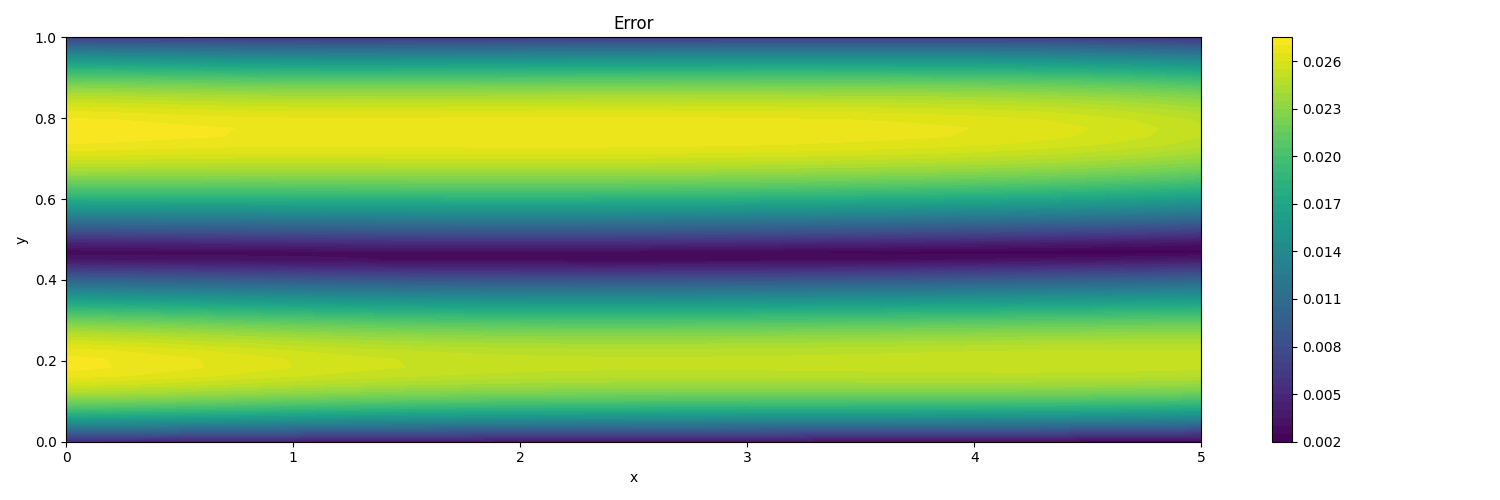
\includegraphics{data/couette_abu_error_best.png}
    \caption{Результат с минимальным показателем отклонения от точного решения в процессе обучения и
    кроссвалидации модели с функцией активации ABU отобраный в результате анализа функции потерь}
    \label{fig:couette_abu_best}
\end{figure}

Однако как было отмечено при кроссвалидации функции потерь, имеется неоднозначность между
функцией потерь для уравнений Навье-Стокса и потерями на границах области. Хоть и были
получены результаты с низким процентом отклонения от точного решения, где максимальное
отклонение составило $2.6\%$, среди кроссвалидируемых результатов были и следующие
качественные модели (табл. \ref{table:couette_abu_best_models})

\begin{table}[ht]
    \centering
    \caption{Качественные модели при разных коэффициентах}
    \begin{tabular}{ |c|c|c|c|c|c| } 
        \hline
        Номер модели & $\beta_0$ & $\beta_1$ & $\beta_2$ & $\beta_3$ & Отклонение, \% \\
        \hline
        $1$ & $1$ & $1$ & $1$ & $0$ & $1.125$ \\ 
        \hline
        $2$ & $1$ & $1$ & $1$ & $0$ & $1.800$ \\ 
        \hline
        $3$ & $1$ & $1$ & $1$ & $0$ & $2.600$ \\ 
        \hline
        $4$ & $1$ & $1$ & $0$ & $0$ & $2.880$ \\ 
        \hline
        $5$ & $1$ & $1$ & $0$ & $0$ & $2.250$ \\ 
        \hline
        $6$ & $0$ & $1$ & $1$ & $1$ & $4.500$ \\ 
        \hline
        $7$ & $0$ & $1$ & $1$ & $1$ & $2.700$ \\ 
        \hline
    \end{tabular}
    \label{table:couette_abu_best_models}
\end{table}

Как можно заметить, некоторые модели имеют одни и те же коэффициенты, но
разные результаты. Это связано с тем, что результат модели также 
зависит от начальной инициализации весов, которая каждый раз
генерируется случайным образом.

Исходя из таблицы \ref{table:couette_abu_best_models} лучшая модель
выдала результат (рис. \ref{fig:couette_abu_best_model}) с максимальным отклонением в $1.125\%$.

\begin{figure}[ht]
    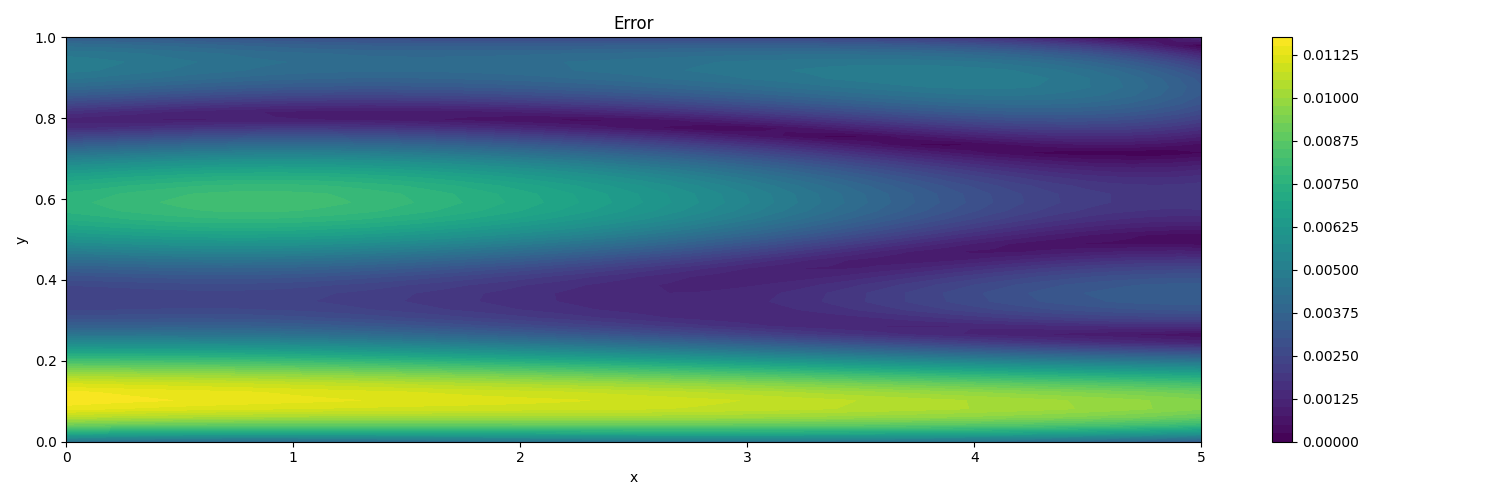
\includegraphics{data/couette_abu_error_best_model.png}
    \caption{Результат с минимальным показателем отклонения от точного решения в процессе обучения и
    кроссвалидации модели с функцией активации ABU отобраный в результате ручного анализа}
    \label{fig:couette_abu_best_model}
\end{figure}

Можно заметить, что оптимизатор и количество слоев совпало
с результатами кроссвалидации, в отличии от параметров
функции активации. Как упоминалось ранее, это связано с
малой выборкой параметров $\beta_i$, а также с присутствием
в выборке плохо обученных моделей. 

\chapter{Заключение}
В процессе анализа поведения физически-информированной нейронной сети были выявлены
закономерности и зависимости от гиперпараметров, на которые следует обращать внимание
при настройке модели для конкретной задачи.

Практическая значимость подхода заключается в уменьшении необходимости в большом объёме
экспериментальных данных, ускорении вычислений и возможности эффективного использования
современных вычислительных платформ (CPU, GPU, NPU). Это открывает перспективы для применения
PINN в таких сферах, как игровая и киноиндустрия, где требуется быстрое и реалистичное
моделирование жидкостей.

В работе проведён анализ влияния различных параметров нейронной сети (структуры, функций
активации, методов оптимизации) на качество решения. Особое внимание уделено выбору
функций активации, показано преимущество адаптивных и комбинированных функций (например,
ABU-PINN) для задач с различными физическими свойствами.

Результаты тестирования на задаче течения Куэтта с известным аналитическим решением подтвердили
способность PINN воспроизводить физически корректные распределения скоростей и давления,
а также выявили влияние архитектурных решений на точность модели.

Выбор правильного оптимизатора позволяет избегать нулевых решений, если это позволяет
функция активации. Количество точек внутри области и на ее границах, а если быть точным,
их отношение, влияет на то, какой из уравнений в постановке задачи будет отдан приоритет.
Конкретного соотношения нет, поэтому следует проводить кроссвалидацию как можно с большим
количеством вариантов. Функция активации в основном влияет на решение внутри области в
силу своей главной задачи --- внести нелинейность. 

Также были сравнены функции активации ABU и REAct, в результате которого были сделаны выводы,
что ABU пусть и медленнее, но намного точнее справляется со своей задачей.

Основные ограничения связаны с необходимостью подбора архитектуры сети под конкретную задачу
и возможной нестабильностью обучения при сложных физических условиях. Тем не менее, подход PINN
демонстрирует высокую гибкость и потенциал для дальнейшего развития.

Физически-информированные нейронные сети являются перспективным инструментом для моделирования
гидродинамических процессов, обеспечивая высокую точность и устойчивость решений при минимальных
требованиях к объёму экспериментальных данных. Дальнейшее развитие этой технологии связано с
оптимизацией архитектур, расширением области применения и интеграцией с другими методами машинного
обучения и численного моделирования.

\printbibliography[title=Список использованных источников] % Автособираемый список литературы


\end{document}